\documentclass[11pt]{article}
%\usepackage{ngerman}
\usepackage[english]{babel}
\usepackage{amsmath,amssymb,amstext}
\usepackage{graphicx}
\usepackage{parskip}
\usepackage{float}
\usepackage{tabularx}
\usepackage{amsmath}
\usepackage{esint}
%\usepackage{subtextbf}
\usepackage{pdfpages}
\usepackage{url}
%\usepackage{cite}
\usepackage{array}
\usepackage{multirow}
\usepackage{hyperref}
\usepackage{biblatex}
\usepackage{todonotes}
\usepackage{subcaption}


 
\bibliography{Documentation/references/references}
\bibliographystyle{plain}
\setlength{\textwidth}{15 true cm}
\setlength{\textheight}{22 true cm}
\oddsidemargin  0.5 cm
\evensidemargin 0.5 cm
\topmargin      0 cm

\renewcommand{\textfraction}{.2}
\renewcommand{\floatpagefraction}{.8}

\begin{document}
%\frontmatter
\pagenumbering{roman}

% Include titlepage
\begin{titlepage}	
	{\sffamily		
		\begin{center}			
			
\includegraphics[width=30mm]{images/TU_Graz_Logo.png}
			
			\vfill\vfill\vfill
			\vfill\vfill\vfill
			
			{Simon Prato}
			% Author with existing titles
			
			\vfill\vfill\vfill
			
			{\LARGE\bfseries{Numerical Investigation of TEM Cells and Antenna Coupling}}
			% Title of the thesis			
			
			\vfill\vfill\vfill
			\vfill\vfill\vfill			
			
			{\bfseries\large{Master Thesis}}
			
			{Studies: {Electrical Engineering}}
						
			\vfill\vfill\vfill			
			
			submitted to
			
			\vfill
			
			{\bfseries\large{Technical University of Graz}}			
			
			\vfill\vfill\vfill			
			
			Supervisor
			
			{Dr. Thomas Bauernfeind}
			
			\vfill
			
			\vfill
			
			
\includegraphics[width=30mm]{Documentation/images/igte_logo.png}
			
			%% OPTIONAL: second supervisor/name of the faculty, etc.
					
			\vfill\vfill\vfill
					
			{Graz}, {August}~{2024}
			
		\end{center}
	}%% end sffamily
\end{titlepage}

\newpage

% Kurzfassung
\iftrue
\cleardoublepage
\setcounter{page}{2}
\vspace*{2.2 cm}
{\Large
\noindent
{\bf Abstract}} \\
\vspace*{0.3 cm}

\noindent

% Abstract
\cleardoublepage
\fi

\selectlanguage{english}
% Inhaltsverzeichnis
	\tableofcontents  

% Tabellenverzeichnis
% optional
\newpage
	\listoffigures 

% Abbildungsverzeichnis
% optinal
\newpage
	\listoftables
	
\cleardoublepage

%\mainmatter
\pagestyle{headings}
\pagenumbering{arabic}

\section{Introduction}

\section{Theoretical Basics}
\subsection{Dipoles}
Modeling the electromagnetic radiation from antennas is a challenging task. Employing magnetic and electric dipoles is an effective approach, particularly for electrically small antennas. They are defined as antennas with dimensions much less than one-tenth of the wavelength ($<<\frac{\lambda}{10}$)\cite{Balanis_1997}. By calculating the respective dipole moments, the coupling between antennas and TEM cells can be numerically estimated. This section provides a brief introduction to the underlying theory of this concept.

\subsubsection{Electric Dipoles}
An electric dipole is often described as two tiny charged metal spheres, which are connected with a linear and thin wire \cite{Griffiths_2024} or simply as an T-antenna containing charged capacitor-plates at the ends of the wire \cite{Balanis_1997}. The distance $d$ between those charges is very short compared to the wavelength ($d << \lambda$).%, therefore the dipole can be approximated as ideal\cite{Griffiths_2024}. 
The electric dipole moment $\mathbf{p}$ is defined by the product of charges and their separation distance, as expressed in \autoref{eqn:elec_dipole_mom}\cite{Balanis_1997,Jackson}. %% Erklärung hier. Besser die Bücher zu referenzieren, als selbst etwas zu erfinden.

\begin{equation}
    \mathbf{p} = \iiint\mathbf{x'} \rho (\mathbf{x'})\mathrm{d}^3x'
    \label{eqn:elec_dipole_mom}
\end{equation}

\autoref{fig:electric_dipole} demonstrates a simple center-fed wire antenna with a narrow gap as the feedpoint. Since the wire is electrically small and very thin, it can be accurately modeled as an electric dipole \cite{Griffiths_2024,Jackson}. A current $I_0$ is injected at the feedpoint, which linearly drops to zero along the antenna arms, as described by \autoref{eqn:current_dipole}\cite{Jackson}.

\begin{equation}
    I(z)= I_0\left( 1-\frac{2|z|}{d} \right)
    \label{eqn:current_dipole}
\end{equation}

%Hier das Ergebnis der Integration anschreiben. Die integration selbst auch anschreiben- 

\begin{figure}[h]
    \centering
    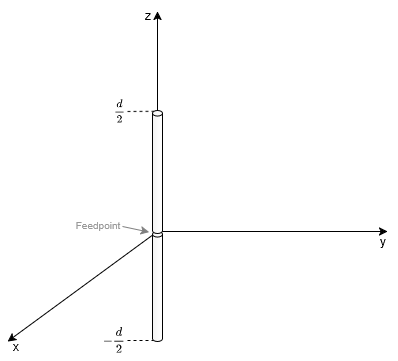
\includegraphics[width=0.5\linewidth]{Documentation//images/electric_dipole_drawing.png}
    \caption{Electric dipole}
    \label{fig:electric_dipole}
\end{figure}

Charge accumulates along the antenna's arms and is expressed as a charge per unit length $\rho'$. The charge distribution $\rho'$ is derived by the continuity equation in frequency domain, as shown in \autoref{eqn:charge_distribution_dipole}. It is uniformly distributed along each antenna arm \cite{Griffiths_2024,Jackson}.

\begin{equation}
    \rho' = \pm\frac{\mathrm{d}}{\mathrm{d}z}\frac{\mathrm{i}I(z)}{\omega} = \pm\frac{2\mathrm{i}I_0}{\omega d}
    \label{eqn:charge_distribution_dipole}
\end{equation}

Knowing the charge distribution $\rho'$ enables the calculation of the electric dipole moment $\mathbf{p}$ using \autoref{eqn:elec_dipole_mom}. This results in \autoref{eqn:dipole_mom_example}. The electric dipole moment $\mathbf{p}$ is parallel to the antenna's arms and points in the z-direction \cite{Griffiths_2024}\cite{Jackson}. 

\begin{equation}
    \mathbf{p}=\int_{-\frac{d}{2}}^{\frac{d}{2}}z\rho'(z)\mathrm{d}z\cdot\mathbf{e}_z = \frac{\mathrm{i}I_0d}{2\omega}
    \label{eqn:dipole_mom_example}
\end{equation}

Next, the vector potential $\mathbf{A}$ is determined. It is generally defined in \autoref{eqn:vector_pot}\cite{Balanis_1997}\cite{Jackson}. % Eventuell extra in einem anderen Kapitel diese Bascis anschreiben. 

\begin{equation}
    \mathbf{A}(\mathbf{x})=\frac{\mu}{4\pi}\frac{\mathrm{e}^{\mathrm{i}kr}}{r}\iiint \mathbf{J}(\mathbf{x'})\mathrm{d}^3x'
    \label{eqn:vector_pot}
\end{equation}

In the case of an electric dipole, the calculations of the vector potential $\mathbf{A}$ simplifies to \autoref{eqn:vector_pot_elec_dipole}\cite{Jackson}.

\begin{equation}
    \mathbf{A} (\mathbf{x})=-\frac{\mathrm{i\mu_0\omega}}{4\pi}\mathbf{p}\frac{\mathrm{e}^{\mathrm{i}kr}}{r}
    \label{eqn:vector_pot_elec_dipole}
\end{equation}
%Should the calculation of fields even be included? I don't need them for research. But the Field equations are important for explaining the frequency behavior of the electric dipole moment. This can be done by the radiation resistance in \autoref{eqn:elec_rad_res}. In our example, the radiation power depends on the frequency squared ($\mathbf{p}$\textasciitilde

Any other field quantities can be derived out of the vector potential $\mathbf{A}$, such as the electric field strength $\mathbf{E}$ and magnetic field strength $\mathbf{H}$. \autoref{eqn:elec_and_mag_field_dipole} expresses their relation \cite{Balanis_1997}. 

\begin{subequation}\label{eqn:elec_and_mag_field_dipole}
    \begin{equation}
    \mathbf{H} = \hat{a}_{\phi} \frac{1}{\mu r} \left[ \frac{\partial}{\partial r} (r A_{\theta}) - \frac{\partial A_{r}}{\partial \theta} \right]
    \end{equation}
    
    \begin{equation}
    \mathbf{E}=-\mathrm{i}\omega\mathbf{A}-\mathrm{i}\frac{1}{\omega\mu\epsilon}\nabla\left(\nabla\cdot\mathbf{A}\right)
    \end{equation}
    
\end{subequation}

The power radiated by an antenna is determined from the time-averaged Poynting vector $ \langle \mathbf{S} \rangle$. \autoref{eqn:time_averaged_poynting} defines this quantity, where only the real part is relevant, since it represents the actual radiated power \cite{Balanis_1997}.

\begin{equation}
    \langle \mathbf{S} \rangle = \frac{1}{2} \, \Re \{ \mathbf{E} \times \mathbf{H}^* \}
    \label{eqn:time_averaged_poynting}
\end{equation}

By integrating the time-averaged Poynting vector $ \langle \mathbf{S} \rangle$ over a closed surface, the radiated power $P_{\mathrm{rad}}$ is determined. The real part of the power is independent of the integrated surface, and in case of an electric dipole is expressed as \autoref{eqn:elec_rad_res}. The radiated power increases with the frequency squared, as the antenna becomes more efficient. This relation holds, as long as the antenna is electrically small.

\begin{equation}
    P_{\mathrm{rad}} = \frac{\mathrm{c}^2\mathrm{Z_0}\mathrm{k}^4}{12\pi}|\mathbf{p}|^2
    \label{eqn:elec_rad_res}
\end{equation}

The electric dipole described in this section approximate the real behavior of electrically short antennas. However, special care must be taken of the excitation method and shape, as it influences the results heavily \cite{Jackson}. Additionally, any antenna investigated through this method must remain as small as possible compared to the wavelength $\lambda$, to reduce any analytical approximation errors. 

The electric field increases quadratically with frequency.... Hence electric dipole moment increases over frequency... Write about that -> Griffiths

\todo{Balanis image theory of dipoles}

% Next, the electric and magnetic fields, how the dipole moment is calculated with this and how ansys HFSS uses this. Look also in the other two ressources, the other two books. Ansys HFSS handles them as physical dipole antennas? Maybe add radiation pattern. Additionally, describe how the electric field odminates in electric dipoles. In Dominik's paper, the magnetic coupling dominates, because of the magnetic dipole.

% The behavior of the electric dipole may be divided into three categories\cite{Griffiths_2024,Jackson}:
% \begin{enumerate}
%     \item The near zone, 
% \end{enumerate}

\subsubsection{Magnetic Dipoles}

The magnetic dipole is modeled as a current loop with radius $b$, whose axis is perpendicular to the plane of the loop. Its radiated fields are analogous to those of an electric dipole, with the electric and magnetic fields interchanged \cite{Balanis_1997}. \autoref{fig:magnetic_dipole_drawing} shows a magnetic dipole.

\begin{figure}[h]
    \centering
    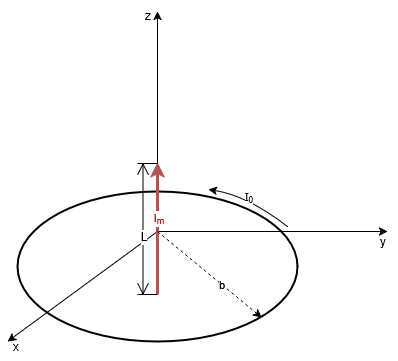
\includegraphics[width=0.5\linewidth]{Documentation//content//10_theory//img/magnetic_dipole_drawing.png}
    \caption{Magnetic dipole}
    \label{fig:magnetic_dipole_drawing}
\end{figure}

The magnetic dipole moment is given by \autoref{eqn:mag_dipole_moment}.

\begin{equation}
    \mathbf{m}=\frac{1}{2}\int (\mathbf{x} \times \mathbf{J})\mathrm{d}^3x
    \label{eqn:mag_dipole_moment}
\end{equation}

A magnetic dipole can be represented with a current loop, or a magnetic current along a straight path. \autoref{eqn:magn_current_curr_loop} shows the relation between these two \cite{Balanis_1997}. 

\begin{equation}
    I_m L = \mathrm{i}S\omega\mu_0 I_0
    \label{eqn:magn_current_curr_loop}
\end{equation}

$I_m$ is the magnetic current with the unit $\mathrm{V}$. The area $S$ of the loop is calculated by $b^2\pi$. $I_0$ is the electric current with the unit $\mathrm{A}$ flowing through the loop, and $\mu_0$ is the permeability of free space.

\todo{Add fields and radiation power formulas, if it is needed later}

\subsubsection{Crossed Dipoles}
% Read Bauernfeind's: Crossed Dipole Antennas

% When placing the magnetic dipole in the center of the upper or lower chamber of the TEM cell, and pointing in y-direction, it will generate a TEM-wave. Same goes for the electric dipole, pointing in z-direction. When combining two of these dipole moments, any excitation with the first order TEM mode is possible. This is the main idea for modeling antennas. The relation of the magnetic and electric fields is assumed to be roughly equal to the free space wave impedance. Also, magnetic dipoles create a difference in output voltage of the two ports, while electric dipoles create a increase of voltage in both ports. The power transmitted is the same. However: How are they modeled in HFSS? 

Crossed dipoles can generate a wide variety of radiation patterns. Supposed two dipoles are placed perpendicular to each other and fed 90° out of phase, an omnidirectional radiation pattern in created \cite{7293591}. If the equivalent dipoles of an EUT represents such two dipoles, any mode which can propagate in the TEM cell will do so, and therefore influence the measurement result. It is therefore not only important to know which dipoles there are representing the EUT, but also what phase and magnitude they have. Meaning that not only the dipoles aligned with the TEM mode alone influence the result. 

% Also, the reflections of the conducting sheets of the TEM cell might enhance the dipoles' gain, therefore artificially supporting a certain mode even more. This property is often used in antennas, where a perfect electric conductor (PEC) is placed a quarter wavelength away from the antenna, hence enhancing the gain \cite{7293591}. 


\subsection{Finite Element Method}

\subsubsection{General Idea}
Problems involving the calculations of electromagnetic fields are often cumbersome and difficult to solve. This is due to the need of solving differential equations describing these fields over a computational domain, which is not possible with a computer in this sense. The simulation software Ansys HFSS (High Frequency Simulation Software) aims to provide a solution. This software is used for the simulations in \autoref{sec:simulations}, hence it is described in this following, dedicated section.

HFSS uses a numerical technique, namely the Finite Element Method (FEM). The general idea of FEM after Rayleigh-Ritz-Galerkin is to choose a number of basis functions. The goal is to find a linear combination of these basis functions, so that the differential equation is satisfied as closely as possible. This turns the problem of solving a differential equation into a system of algebraic equations, which the computer can process. There is always a set of basis functions which enable the calculation to converge to the real solution. However, the number of basis functions used in the domain is limited, due to reasons of computability \cite{STRANG_2018}. 

FEM therefore divides the domain into finite elements, i.e. smaller pieces. Then, within each piece, such a basis function is assigned. A linear combination of these basis functions are found, which satisfy the differential equations. In region where the approximating solution has a high degree of error, the accuracy may be increased by further subdividing the finite elements. This is repeated, until the error falls below a certain threshold, and a precise solution is derived.

\subsubsection{Dividing a computational domain into finite elements}

The differential equation to be solved is shown in \autoref{eqn:full_wave_equation}, where $\epsilon_r$ is the relative permeability and $\mu_r$ is the relative permeability of the material. The variable $k_0$ is the wave number of free space and equals $k_0=\omega\sqrt{\epsilon_0\mu_0}$. \cite{Cendes_Lee_1988,85399,Cendes_1991}.

\begin{equation}
    \nabla\times\left(\frac{1}{\mu_r}\nabla\times\mathbf{E}\right)-k_0^2\epsilon_r\mathbf{E}=0 \quad\text{in $\Omega$}
    \label{eqn:full_wave_equation}
\end{equation}

This equation is solved in a computational domain $\Omega$. This computational domain is divided into finite elements, called a mesh. Each node in this mesh has polynomial functions assigned, which are weighted to approximate the real solution. It has been proven that tetrahedral finite elements are best suited for this task, as they are geometrically flexible and make the definition of complete polynomial approximation functions possible \cite{Shenton_Cendes_1985}. Ansys HFSS uses a adaptive finite element mesh generator, which automatically provides a mesh for a given 3-dimensional construction. The Delaunay tesselation for three-dimensions is used for generating a mesh. It efficiently creates a mesh from objects of arbitrary shapes. Any boundary condition can be added recursively to the mesh. At the heart of this algorithm lies the property, that the circumsphere of an tetrahedra's vertices may not contain other tetrahedra's vertices. 

\autoref{fig:tetrahedral_mesh} shows one of such tetrahedrons. At the edge points, the components of the field which are normal to the respective edge and tangential to the face of the element is stored. At the vertex points, the component of a field which are tangential to the edges are stored. The value of the field at any midpoint is derived through interpolation from the node values. The basis function is used for interpolation.

\begin{figure}[h]
    \centering
    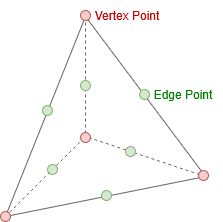
\includegraphics[width=0.25\linewidth]{Documentation/content/10_theory/img/tetrahedral_mesh.png}
    \caption{Tetrahedron with points on the edge and vertices.}
    \label{fig:tetrahedral_mesh}
\end{figure}

Because of the way how the fields are stored in the tetrahedra, they are called tangetial vector finite elements. Their advantage is that tangential components of fields can be forced to be equal among adjacent tetrahedra at the boundary. For example, an electric field stored at a vertex point must point in the direction along one of the edges, therefore it is tangential to the element. An adjacent element then has the same tangential electric field imposed at this node, leading to a continuous tangential electric field, therefore satisfying the boundary conditions implied by the Maxwell equation automatically. Furthermore, any Dirichlet boundary conditions can easily be set along the edges.
\cite{85399}. 

The finite element is described as \autoref{eqn:finite_element_3d}, where $L_2(\Omega)$ is a set of square integrable functions and $P_1$ a set of piecewise linear functions in the discretized domain $\Omega$ \cite{104986}. The vector fields at the vertices are given as $u$. $D(\Omega)$ is a set of divergence free functions. The vectors $u$ used in the finite element therefore 

\begin{itemize}
    \item are continuous in the normal direction.
    \item are square integrable.
    \item have a curl describable by piecewise linear functions.
\end{itemize}

\begin{equation}
    H^{(\dim=3)}_1(\mathrm{curl}) = \left\{ \mathbf{u} \mid \mathbf{u} \in \left[ L_2(\Omega) \right]^3, \nabla \times \mathbf{u} \in \left[ P_1(\Omega) \right]^3 \cap D(\Omega) \right\}
    \label{eqn:finite_element_3d}
\end{equation}

\autoref{fig:tetrahedra_w_unknowns} shows the finite element with the unknowns marked at each point. For reasons of simplicity, only the face is shown. The variables $u_i^j$ and $u_j^i$ are imposed across element boundaries, therefore guaranteeing tangential continuity at boundaries. Additionally, they inherently defined a linear polynomial, meaning that they describe a gradient of the field along this edge. \autoref{eqn:tangential_vector_component} describes this relation mathematically, where $\mathbf{t}_{ij}$ is the unit vector tangentially to the edge from node i to node j and $l_{ij}$ is the length of this edge.

\begin{equation}
    \mathbf{u}\cdot\mathbf{t}_{ij}=\frac{1}{l_{ij}}\left( u_i^j-u_j^i \right)
    \label{eqn:tangential_vector_component}
\end{equation}

\begin{figure}[h]
    \centering
    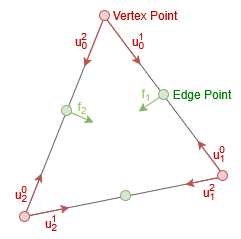
\includegraphics[width=0.25\linewidth]{Documentation//content//10_theory/img/tetrahedra_w_unknowns.png}
    \caption{Face of the finite element with unknowns}
    \label{fig:tetrahedra_w_unknowns}
\end{figure}

Two facial unknowns $f_1$ and $f_2$ are added to two of the three edge points at one face. Contrary to the variables $u_i^j$, the facial unknowns $f_i$ are only assigned locally at each element and do not cross boundaries. The purpose of the facial unknowns $f$ is to provide a quadratic polynomial for the field component normal to the edges. This will lead to a linear approximation for the curl of the unknown vector field $\nabla\times \mathbf{u}$, providing sufficient accuracy. The overall vector field of this element is then calculated by a superposition of all nodes' vector attributions.

\subsubsection{Solving the differential equation}

A testing function $\mathbf{W}_n$ is defined, which is multiplied to \autoref{eqn:full_wave_equation}. Integrating over the whole test volume then leads to \autoref{eqn:test_funct}. This yields $N$ equations, with $n=1,2,...N$, for each finite element in the domain $\Omega$. This is a common procedure in FEM, and it works through orthogonalization of the residual of \autoref{eqn:full_wave_equation} with respect to the function $\mathbf{W}_n$. This means the new goal of the solution is to minimize the residual by making $\mathbf{W}_n$ as orthogonal as possible \cite{Mohsen_1982}.

\begin{equation}
    \int_\Omega\left( \mathbf{W}_n\cdot\nabla \times\left( \frac{1}{\mu_r}\nabla\times\mathbf{E} \right)-k_0^2\epsilon_r\mathbf{W}_n\cdot\mathbf{E} \right)\mathrm{d}V=0
    \label{eqn:test_funct}
\end{equation}

Using the vector identity $\nabla\cdot\left(\mathbf{a}\times\mathbf{b}\right)=\left(\nabla\times\mathbf{a}\right)\cdot\mathbf{b}-\mathbf{a}\cdot\left(\nabla\times\mathbf{b}\right)$  on \autoref{eqn:test_funct} provides a weak form of the equation, meaning a form of the original partial differential equation, which does not contain all original derivatives \cite{Cendes_Lee_1988,Cendes_1991}. Additionally, boundary terms come into play, as seen in the right hand side of the resulting \autoref{eqn:greens_theorem_wave_eqn}. The usefulness in this step has been described as lowering the highest-order derivative, therefore the approximating functions need to guarantee continuity of value, not of slope \cite{huebner2001finite}. Another explanation is the possibility of incorporation of Neumann boundary conditions \cite{Mohsen_1982}. 

\begin{equation}
    \int_\Omega \left[ \left(\nabla \times \mathbf{W}_n \right)\cdot \frac{1}{\mu_r}\nabla\times \mathbf{E}-k_0^2\epsilon_r\mathbf{W}_n\cdot\mathbf{E}\right]\mathrm{d}V=\underbrace{\oint_{\partial\Omega}\left( \mathbf{W}_n\times \frac{1}{\mu_r}\nabla\times\mathbf{E}\right)\cdot\mathrm{d}\mathbf{S}}_{\text{Boundary term}}
    \label{eqn:greens_theorem_wave_eqn}
\end{equation}

Next, the electric field $\mathbf{E}$ is represented by a superposition of basis functions. When applying Galerkin's method, the basis functions are equal to the test functions $W_n$. \autoref{eqn:representation_e_field_fem} demonstrates the sum of the basis functions, which are weighted with the variable $x_m$. These variables $x$ for all elements have to be solved, to find the electric field $\mathbf{E}$ over the whole domain. The FEM has therefore reduced the initial wave equation in \autoref{eqn:full_wave_equation} to a simple linear matrix equation $Ax=b$, where $A$ is a known $N\times N$ matrix, $b$ contains port excitations and $x$ is the unknown. Ideally, the basis functions are defined to be zero outside of their adjacent elements. This will result to zero for all entries in the matrix, where the test and basis function do not overlap. Therefore, the matrix is sparse, and will be solved much faster. In the end, other electromagnetic quantities can all be derived through the electric field.

\begin{equation}
    \mathbf{E}=\sum^N_mx_m\mathbf{W}_n
    \label{eqn:representation_e_field_fem}
\end{equation}

\autoref{eqn:matrix_a} shows what the matrix then looks like. Some manipulation on the boundary term have been made, so that it contains the surface impedance $Z_s$. The surface impedance defines the ratio of the electric field to the magnetic field on the boundary region. Furthermore, it contains the free space, which equals $\eta_0 \approx 377\,\Omega$.

\begin{equation}
A_{ij} = \int_{\Omega} \nabla \times \mathbf{W}_i \, \frac{1}{\mu_r} \nabla \times \mathbf{W}_j \, \mathrm{d}V 
- k_0^2 \int_{\Omega} \mathbf{W}_i \, \varepsilon_r \mathbf{W}_j \, \mathrm{d}V 
+ \mathrm{i} k_0 \left(\frac{\eta_0}{Z_s}\right) \oint_{\partial\Omega} \mathbf{n} \times \mathbf{W}_i \cdot \mathbf{n} \times \mathbf{W}_j \, \mathrm{d}\mathbf{S}
\label{eqn:matrix_a}
\end{equation}

\subsubsection{Adaptive solution process}

Each finite element therefore has a solved electric field assigned, which should approximate the real solution as closely as possible. To determine the error for each element, \autoref{eqn:full_wave_equation} is evaluated. The elements with the highest residuals contain the largest deviation from the real result, meaning they have a large degree of error. Region in the mesh with large degrees of errors are refined, i.e. the tetrahedral finite elements are split into smaller ones. This allows the FEM solver to recalculate the fields in this region with higher precision, leading to a smaller residual. Consequently, the finite elements represent the fields more accurately, due to a smaller element size and higher resolution \cite{1063929}. An additional method is increasing the order of the polynomial basis functions of elements with low degree of accuracy.

\begin{equation}
    \nabla\times\left(\frac{1}{\mu_r}\nabla\times\mathbf{E}_{\mathrm{solved}}\right)-k_0^2\epsilon_r\mathbf{E}_{\mathrm{solved}}=residual
    \label{eqn:full_wave_equation_solved}
\end{equation}

To determine when the iterative refinement process is done and the solution good enough, some kind of threshold must be defined. One possibility is the $\mathrm{Max}\ \Delta \mathrm{S}$ parameter. It is compared to the difference of S-parameters of the defined excitation ports over two iterations. If, after a mesh refinement, the S-parameters of the ports do not significantly change anymore, meaning change less than $\mathrm{Max}\ \Delta \mathrm{S}$, then the iterative process can be considered done. This described iterative process is shown in \autoref{fig:workflow_fem}. 

\begin{figure}[h]
    \centering
    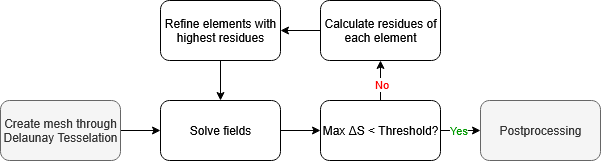
\includegraphics[width=0.75\linewidth]{Documentation//content//20_antennas//img/workflow_fem.png}
    \caption{Adaptive solution process}
    \label{fig:workflow_fem}
\end{figure}

\todo{Short HFSS introduction with boundary conditions, ports and modal and terminal solutions}
 % Fehlende Ressourcen von Zoltan in Journal of Applied Physics. Schreibe über mathetmaische Grundlagen, Meshing, Dipole Excitation und Impedance Network Boundary Counditions (INBC)

% Additional missing ressource: Finite Elements, Electromagnetics, and Design



\subsection{Lorentz Reciprocity Theorem}

The Lorentz reciprocity theorem proves to be very useful, hence it is summarized here. It states that any two fields $\mathbf{E_1}$, $\mathbf{H_1}$ and $\mathbf{E_2}$, $\mathbf{H_2}$, which are of the same frequency and in linear and isotropic media, can be expressed by its differential form in \autoref{eqn:lorentz_rec_theorem} \cite{Balanis_1997,Collin_2015}. Here, $\mathbf{J}$ describes the electric current density with the unit $\frac{\mathrm{A}}{\mathrm{m^2}}$ and $\mathbf{M}$ the magnetic current density with the unit $\frac{\mathrm{V}}{\mathrm{m^2}}$. They act as sources, exciting the electric and magnetic fields $\mathbf{E}$ and $\mathbf{H}$. The theorem says, that under the previously described conditions, any source and response can be locally interchanged, and the results would remain the same.

\begin{equation}
    -\nabla \cdot (\mathbf{E_1}\times \mathbf{H_2}-\mathbf{E_2}\times \mathbf{H_1})=\mathbf{E_1}\cdot \mathbf{J_2}+\mathbf{H_2}\cdot \mathbf{M_1}-\mathbf{E_2}\cdot \mathbf{J_1}-\mathbf{H_1}\cdot \mathbf{M_2}
    \label{eqn:lorentz_rec_theorem}
\end{equation}

By taking a volume integral of both sides of \autoref{eqn:lorentz_rec_theorem} and using the divergence theorem, \autoref{eqn:lorentz_rec_theorem_int} emerges \cite{Balanis_1997,Collin_2015}.

\begin{equation}
    \oiint (\mathbf{E_1}\times \mathbf{H_2}-\mathbf{E_2}\times \mathbf{H_1})\cdot \mathrm{d}S\mathbf{n}=\iiint
\mathbf{E_1}\cdot \mathbf{J_2}+\mathbf{H_2}\cdot \mathbf{M_1}-\mathbf{E_2}\cdot \mathbf{J_1}-\mathbf{H_1}\cdot \mathbf{M_2}\cdot \mathrm{d}V
    \label{eqn:lorentz_rec_theorem_int}
\end{equation}

If there aren't any sources present, meaning that $\mathbf{J_1}=\mathbf{J_2}=\mathbf{M_1}=\mathbf{M_2}=0$, the Lorentz reciprocity theorem simplifies to \autoref{eqn:lorentz_rec_theorem_wo_sources} \cite{Balanis_1997,Lorrain_Corson_1970}. This is especially useful for free wave propagation of antennas.

\begin{equation}
    -\nabla \cdot (\mathbf{E_1}\times \mathbf{H_2}-\mathbf{E_2}\times \mathbf{H_1})=0
    \label{eqn:lorentz_rec_theorem_wo_sources}
\end{equation}

Another application arises when investigating a volume $V$ confined by a perfectly conducting surface $S$, through which to linear current densities $\mathbf{J_1}$ and $\mathbf{J_2}$ flow. Because $\mathbf{n}\times\mathbf{E_1}=\mathbf{n}\times\mathbf{E_2}=0$ along the surface $S$, the surface integral in \autoref{eqn:lorentz_rec_theorem_int} equals zero, and \autoref{eqn:rayleigh_carson} arises. This is the Rayleigh-Carson from of the Lorentz reciprocity theorem and is particularly useful for deriving waveguide modes and constructing the respective fields \cite{Collin_2015}.

\begin{equation}
    \mathbf{E_1}\cdot\mathbf{J_2}=\mathbf{E_2}\cdot\mathbf{J_1}
    \label{eqn:rayleigh_carson}
\end{equation}

% This will be used to model dipoles with Green's Theorem in waveguides.

\subsection{Green's Function}

Green's function describes the response of a linear differential operator L to a point source, described with a delta-function $\delta$. The general form is shown in \autoref{eqn:general_greens_funct}. 

\begin{equation}
    \mathrm{L}G(\mathbf{x},\mathbf{x'}) = \delta(\mathbf{x}-\mathbf{x'})
    \label{eqn:general_greens_funct}
\end{equation}

Once \autoref{eqn:general_greens_funct} is solved and the Green's function $G$ of this specific operator is known, it can be used to solve any function, like $u(\mathbf{x})$ in \autoref{eqn:examplary_function_with_operator}, on which this operator is used on, by superposition. The resulting \autoref{eqn:examplary_function_solved} solves for $u(\mathbf{x})$ by using a convolution integral with the Green's function and the source function $f(\mathbf{x})$.

\begin{subequations}
\begin{equation}
    Lu(\mathbf{x}) = f(\mathbf{x})
    \label{eqn:examplary_function_with_operator}
\end{equation}

\begin{equation}
    u(\mathbf{x})=\int G(\mathbf{x},\mathbf{x'})f(\mathbf{x'})\mathrm{d}\mathbf{x'}
    \label{eqn:examplary_function_solved}
\end{equation}
\end{subequations}

For example, it is commonly used to solve equations containing the Nabla operator $\nabla$ in electrostatics. \autoref{eqn:greens_function_scalar_pot_1} and \autoref{eqn:greens_function_scalar_pot_2} demonstrate how the scalar potential $\phi$ can be calculated with point sources in space $\rho$ just by knowing the Green's function of the Nabla operator, which is $G(\mathbf{x},\mathbf{x'}) = \frac{1}{4\pi |\mathbf{x}-\mathbf{x'|}}$.

\begin{subequations}
\begin{equation}
    \nabla \phi = -\frac{\rho}{\epsilon_0}
    \label{eqn:greens_function_scalar_pot_1}
\end{equation}
\begin{equation}
    \phi(\mathbf{x}) = \frac{1}{4\pi\epsilon_0}\iiint_V\frac{\rho(\mathbf{x'})}{|\mathbf{x}-\mathbf{x'}|}\mathrm{d}V'
    \label{eqn:greens_function_scalar_pot_2}
\end{equation}
\end{subequations}

When boundary conditions are present, the Green's function may be modified to make the boundary condition vanish. Same goes for the dyadic Green's function, where the boundary condition are considered to create a taylored Green's function. This enables an expansion of the fields in a waveguide excited by an internal source. The perfectly conducting surfaces of the waveguides mirror the source infinitely often. Therefore, the Green's function may be represented by a series of these mirror sources. In practice, these calculations are cumbersome, and only the most significant parts of the series are computed \cite{Collin_2015}. %Should I show mathematical calculations?

\todo{dyadic green's function, which just maps the coordinates to each other.}

% Read more about Green's function with the Collin book. Then, solve one Green's function for a dipole in a waveguide with normal modes and Lorentz Reciprocity Theorem.



\subsection{Numerical Investigation of Propagating Modes in TEM Cells}\label{sec:modes_tem_cell}
\subsubsection{Mathematical derivation}
% Goal is to describe the modes in a TEM cell, including their cut-off frequencies. \cite{Kreindl_Bauernfeind_Weiss_Stockreitner_Kaltenbacher_2024} shows that these investigations are important. There are also modes propagating perpendicular to the intended propagation direction. Why are no waveguides used? Explain.

% In this paper, a VCSEL with a decoupling capacitor are modeled. It is visible, that the electric coupling dominates at an orientation of 90°. A local minimum is then visible. At 400\,MHz and upwards, inductive coupling becomes dominant, but only at 0° where it couples with the septum. It is possible, that a certain mode can propagate at a certain frequency, which influenced the result in this paper. 


Any electromagnetic field distribution in a waveguide can be represented by an infinite series of normal modes. \autoref{eqn:norm_power} shows that each mode is orthogonal to each other, with $\mathbf{e_n}^\pm$ and $\mathbf{h_n^\pm}$ being the function vectors of the electric and magnetic field in transverse direction \cite{Collin_2015}. A coupling between the modes only occurs due to geometric changes of the waveguide. Additionally, each mode is normalized to $\sqrt{\mathrm{W}}$, shown by \autoref{eqn:unit_power}. Only the transverse fields are investigated in these Equations, because they carry power along the waveguide, opposed to the fields in the propagation direction.

\begin{align}
    \iint \mathbf{e_n^\pm}\times \mathbf{h_m^\pm}\mathrm{d}S\mathbf{n}&=0 \quad\text{if}\quad n\neq m
    \label{eqn:norm_power}\\
    \iint \mathbf{e_n^\pm}\times \mathbf{h_n^\pm}\mathrm{d}S\mathbf{n}&=1
    \label{eqn:unit_power}
\end{align}

The radiated fields can be described by a summation of normal modes, as in \autoref{eqn:modal_superposition1} and \autoref{eqn:modal_superposition2}. The coefficients of these modes are straightforward to calculate, due to Lorentz Reciprocity Theorem, if the waveguide's walls are perfectly conducting. Ideally, any higher order mode than the first TEM mode will be suppressed, and the calculation simplifies to $n=0$. Additionally, it is assumed that the source is electrically small, which makes it possible to represent it with dipoles, further simplifying the equations \cite{Koepke_1989}. 

\begin{align}
    \mathbf{E^\pm}&=\sum_na_n\mathbf{E_n^\pm}    \label{eqn:modal_superposition1}\\
    \mathbf{H^\pm}&=\sum_na_n\mathbf{H_n^\pm}    \label{eqn:modal_superposition2}
\end{align}

Suppose a current source $\mathbf{J_1}$ excites a waveguide (as is the case with the dipoles in the TEM cell). Normally, such a current source would be driven with external fields, but for the sake of the argument, they are ignored. Only $\mathbf{E}$ and $\mathbf{H}$ are considered, which are the fields radiated by $\mathbf{J_1}$. Additionally, $\mathbf{E}_n^\pm$ and $\mathbf{H}_n^\pm$ are the resulting waveguide fields, with the signs indicating the direction of propagation. Take \autoref{eqn:lorentz_rec_theorem_int} and set $\mathbf{J_2}=\mathbf{M_1}=\mathbf{M_2}=0$. Now, only the current source $\mathbf{J_1}$ remains, and the \autoref{eqn:J1_propagating_waves} emerges. % Explain how certain surfaces do not to have be integrated, therefore rendering this equation very useful. Also, the expansion coefficients can be determined. Maybe do this calculation with a rectangular waveguide.

\begin{equation}
    \oiint _S (\mathbf{E_n^\pm}\times \mathbf{H}-\mathbf{E}\times \mathbf{H}_n^\pm)\cdot\mathrm{d}\mathbf{S}=\iiint \mathbf{J_1}\cdot\mathbf{E_n^\pm}\mathrm{d}V
    \label{eqn:J1_propagating_waves}
\end{equation}

In case of the TEM cell, it is desirable that only the TEM mode is propagating, and that the source is represented by a dipole. Considering an electric dipole, therefore, the \autoref{eqn:dipole_tem_waves} arises. In this equation, the wave amplitudes $a$ and $b$ are given through the surface integral in the Lorentz Reciprocity theorem, with $a$ being the wave going to the left side, and $b$ to the other. The electric dipole moment $\mathbf{e_m}$ is given by the current $\mathbf{J}$ flowing through the infinitesimal wire. Note that only the electric field of TEM wave propagation is considered. In reality, more modes may propagate, for which the electric field must be replaced by the superposition of normal modes as in \autoref{eqn:modal_superposition1}. %Additionally, to calculate the exact value of the electric field, a series of image sources as a Green's function may be applied.

\begin{equation}
\begin{pmatrix}a \\b\end{pmatrix} = -\frac{1}{2}\mathbf{m_e}\cdot \mathbf{E}^\pm
\label{eqn:dipole_tem_waves}
\end{equation}

If this arbitrary current distribution forms an infinitesimal loop, the source can be represented by a magnetic dipole. This leads to \autoref{eqn:mag_dipole_moment_tem}. The requirement for this formulation to work, is that the magnetic fields $\mathbf{H}^\pm$ does not change over the loop area, i.e. the loop is electrically small \cite{Collin_2015,Sreenivasiah_Chang_Ma_1981}.

\begin{align}
    \begin{pmatrix}a \\b\end{pmatrix} &= -\oint_C \mathbf{E}^\pm \mathrm{d}l \nonumber \\
    &= -\iint_{S_0} \nabla \times \mathbf{E}^\pm \mathrm{d}\mathbf{S}\nonumber\\
    &= \mathrm{i}\omega\mu_0\iint_{S_0} \mathbf{H}^\pm\cdot \mathrm{d}\mathbf{S}\nonumber\\
    &= \mathrm{i}\omega\mu_0\mathbf{m}_m\mathbf{H}^\pm 
    \label{eqn:mag_dipole_moment_tem}
\end{align}


If there are several modes propagating, it is useful to find the coefficients of the modes $a_n$ and $b_n$ in \autoref{eqn:modal_superposition1} and \autoref{eqn:modal_superposition2}. In this case, the orthogonality property in \autoref{eqn:norm_power} is used to derive \autoref{eqn:an} and \autoref{eqn:bn} \cite{Collin_2015}. The wire is described by a curve C, and the tangential vector $\boldsymbol{\tau}$ is used to integrate along this curve.

\begin{subequations}
    \begin{equation}
        2a_n = -\int_C \boldsymbol{\tau}\cdot\mathbf{E}_n^-\mathrm{d}l
        \label{eqn:an}
    \end{equation}
        \begin{equation}
        2b_n = \int_C \boldsymbol{\tau}\cdot\mathbf{E}_n^+\mathrm{d}l
        \label{eqn:bn}
    \end{equation}
\end{subequations}

\subsubsection{Modes in TEM cell}

A TEM cell is often used for EMC test specifications, as it enables the propagation of TEM waves, which resemble planar free-space waves. Additionally, it shields the waves from radiating to the sides, for which it has a clear advantage to a stripline \cite{809846,990711}. A simple rectangular waveguide cannot be used for this application. Assuming that a monochromatic wave traveling down the waveguide, the waves will propagate without dampening only at a certain angle of reflection on the perfectly conducting surface. A short mathematical proof can be shown here, using Maxwell's equation. It shows that the electric and magnetic fields in direction of propagation cannot both be zero. % Continue with some calculations, showing that TEM wave propagation is not possible?
\begin{align}
    \mathbf{E}&=(E_{0,x}\cdot\mathbf{e_x}+E_{0,y}\cdot\mathbf{e_y}+E_{0,z}\cdot\mathbf{e_z})\mathrm{e}^{\mathrm{i}(\omega t-kz)}\\
    \mathbf{H}&=(H_{0,x}\cdot\mathbf{e_x}+H_{0,y}\cdot\mathbf{e_y}+H_{0,z}\cdot\mathbf{e_z})\mathrm{e}^{\mathrm{i}(\omega t-kz)}\\
    \nabla \times \mathbf{E} &=\begin{pmatrix}\frac{\mathrm{d}}{\mathrm{d}y}E_z-\mathrm{i}kE_y \\\mathrm{i}kE_x-\frac{\mathrm{d}}{\mathrm{d}x}E_z \\\frac{\mathrm{d}}{\mathrm{d}x}E_y-\frac{\mathrm{d}}{\mathrm{d}y}E_x\end{pmatrix}=\begin{pmatrix} -\mathrm{i}\omega B_x\\-\mathrm{i}\omega B_y\\ -\mathrm{i}\omega B_z \end{pmatrix}\\
    \nabla \times \mathbf{B} &=\begin{pmatrix}\frac{\mathrm{d}}{\mathrm{d}y}B_z-\mathrm{i}kB_y \\\mathrm{i}kB_x-\frac{\mathrm{d}}{\mathrm{d}x}B_z \\\frac{\mathrm{d}}{\mathrm{d}x}B_y-\frac{\mathrm{d}}{\mathrm{d}y}B_x\end{pmatrix}=\begin{pmatrix} \frac{\mathrm{i}\omega}{\mu\epsilon} E_x\\\frac{\mathrm{i}\omega}{\mu\epsilon} E_y\\ \frac{\mathrm{i}\omega}{\mu\epsilon} E_z \end{pmatrix}
\end{align}

If $E_z$ and $B_z$, the fields in direction of propagation, were both zero, then the change of the transverse fields would be constantly zero, and because of the boundary conditions, all transverse fields would be zero. \autoref{eqn:rect_waveguide_gauss} shows Gauss' law and \autoref{eqn:rect_waveguide_faraday} Faraday's law if $E_z=B_z=0$, from which the unchanging transverse electric field can be derived. 

\begin{align}
    \frac{\mathrm{d}}{\mathrm{d}x}E_x+\frac{\mathrm{d}}{\mathrm{d}y}E_y&=0\quad\text{Derived out of Gauss' law}\label{eqn:rect_waveguide_gauss}\\
    \frac{\mathrm{d}}{\mathrm{d}y}E_x-\frac{\mathrm{d}}{\mathrm{d}x}E_y&=0\quad\text{Derived out of Faraday's law}\label{eqn:rect_waveguide_faraday}
\end{align}

A TEM cell solves this problem, by having a gap between the septum and the side walls. Essentially, it can be considered as two rectangular waveguides with apertures on the sides. Those apertures allow perturbations of the electromagnetic fields between them. The boundary conditions of the Laplace equation now changed due to the gaps. The Green's function may be calculated of the new construction, now considering the boundary conditions at the gaps, which must be the same for both waveguides (to prevent discontinuities). In the papers of Tippet, Chang and Wilson, this new Green's function lead to the excitation of TEM modes in both waveguides \cite{Tippet_Chang_Crawford_1976,Wilson_1981}.

\todo{Maybe calculate with Green's function as in \cite{4091747}. The resulting radiation resistance might also be helpful later to interpret simulation results.}
% To do this, the electric and magnetic field are described by the wave equations in \autoref{eqn:wave_equ_e_field} and \autoref{eqn:wave_equ_h_field} \cite{Collin_2015}. 

% \begin{subequations}
% \begin{equation}
%     \left(\nabla^2-\mu\epsilon\frac{\mathrm{d^2}}{\mathrm{d}t^2}\right)\mathbf{E}(\mathbf{x})=\mu\frac{\mathrm{d}}{\mathrm{d}t}\mathbf{J}+\frac{\nabla\rho}{\epsilon}
%     \label{eqn:wave_equ_e_field}
% \end{equation}

% \begin{equation}
%     \left(\nabla^2-\mu\epsilon\frac{\mathrm{d^2}}{\mathrm{d}t^2}\right)\mathbf{H}(\mathbf{x})=-\nabla\times\mathbf{J}
%     \label{eqn:wave_equ_h_field}
% \end{equation}
% \end{subequations}

% The Green's function must solve these wave equations, therefore it is formulated as \autoref{eqn:greens_function_wave_equ}. The boundary condition for the Green's function is $\frac{\mathrm{d}}{\mathrm{d}\mathbf{n}}\mathbf{G}=0$, which sets the normal derivative at the boundary to zero. ACHTUNG: ICH GLAUBE, DASS DAS NUR IM FALL \cite{Wilson_1981} FUNKTIONIERT, IN WELCHEM NUR DIE Z KOMPONENTEN BEACHTET WERDEN. DIESE ÄNDERN SICH NICHT ÜBER DIE GAP. This boundary condition applies everywhere, meaning to every conducting surface, as well as the gaps between the septum and the walls of the TEM cell. Consequently, any discontinuities in fields are prevented.

% \begin{equation}
%     \left(\nabla^2-\mu\epsilon\frac{\mathrm{d^2}}{\mathrm{d}t^2}\right)\mathbf{G}(\mathbf{x}-\mathbf{x'})=-\delta(\mathbf{x}-\mathbf{x'})
%     \label{eqn:greens_function_wave_equ}
% \end{equation}

% The solution to this given problem has been solved before \cite{Collin_2015}. Here, the TE guide mode expansion in \autoref{eqn:greens_function_rect_waveguide_solved} are included \cite{Wilson_1981}. THIS IS ONLY Z-COMPONENT OF FIELDS! THERE IS NO VECTOR.

% \begin{equation}
%     \mathbf{G}(\mathbf{x}-\mathbf{x'})=\left(\frac{2}{ab}\right)\sum^\infty_{m,n=0}\frac{\Delta_m\Delta_n}{(K^2_{mn}-k^2)}\cos{\left( \frac{m\pi}{2a}(x+a) \right)}\cos{\left( \frac{m\pi}{2a}(x'+a) \right)}\cos{\left( \frac{n\pi y}{b}\right)}\cos{\left( \frac{n\pi y'}{b}\right)}
%     \label{eqn:greens_function_rect_waveguide_solved}
% \end{equation}

% \begin{itemize}
%     \item $\mathbf{x}$ is the observation point
%     \item $\mathbf{x'}$ is the source point
%     \item $a$ and $b$ are the height and width of the rectangular waveguide
%     \item $m, n$ are the indices of the TE mode
%     \item $x$ is the x-component of the observation point $\mathbf{x}$
%     \item $y$ is the y-component of the observation point $\mathbf{x}$
%     \item $x'$ is the x-component of the source point $\mathbf{x}$
%     \item $y'$ is the y-component of the source point $\mathbf{x}$
%     \item $K_{mn} = \left[ \left( \frac{m\pi}{2a} \right)^2+\left( \frac{n\pi}{b} \right)^2 \right]^{1/2}$
%     \item $k$ is the wave number $\frac{2\pi}{\lambda}$
%     \item $\Delta_m=\begin{cases}1/2, & \text{if } m = 0 \\1,       & \text{if } m \neq 0\end{cases}$ and $\Delta_n=\begin{cases}1/2, & \text{if } n = 0 \\1,       & \text{if } n \neq 0\end{cases}$
% \end{itemize}

% To use the Green's function to solve the magnetic fields, \autoref{eqn:wave_equ_h_field} is multiplied with the Green's function $\mathbf{G}(\mathbf{x}-\mathbf{x'})$, and \autoref{eqn:greens_function_wave_equ} with the magnetic field $\mathbf{H}(\mathbf{x})$. The two resulting equations are subtracted from each other, which leads to \autoref{}.

% \begin{equation}
%     \mathbf{G}(\mathbf{x}-\mathbf{x'})\frac{\mathrm{d^2}}{\mathrm{d}t^2}\mathbf{H}(\mathbf{x})-\mathbf{H}(\mathbf{x})\frac{\mathrm{d^2}}{\mathrm{d}t^2}\mathbf{G}(\mathbf{x}-\mathbf{x'})=-\mathbf{G}(\mathbf{x}-\mathbf{x'})\nabla\times\mathbf{J}(\mathbf{x})+\mathbf{H}(
% \end{equation}


The TEM cell used in the simulation has a width of $a=200\,\mathrm{mm}$ and a height of $b=100\,\mathrm{mm}$. A cross section of the TEM cell with the important dimensions is shown in \autoref{fig:tem_cell_crosssection}. The cutoff frequencies of the higher order TE and TM modes can be approximated by the same formula, shown in \autoref{eqn:cutoff_frequency_rect_waveguide} for rectangular waveguides. However, this is only true, if the septum is very thin ($t/b << 0.1$), and for modes with n-even subscripts, i.e. TE\textsubscript{m,2n} and TM\textsubscript{m,2n} modes.

\begin{figure}[h]
    \centering
    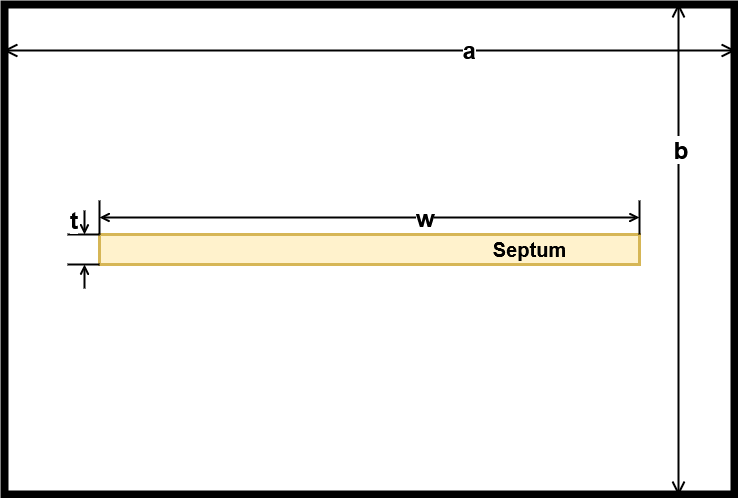
\includegraphics[width=0.5\linewidth]{Documentation//content//10_theory//img/tem_cell_crosssection.png}
    \caption{Cross section of the TEM cell}
    \label{fig:tem_cell_crosssection}
\end{figure}

\begin{equation}
    f_c = \frac{c}{2} \sqrt{\left(\frac{m}{a}\right)^2 + \left(\frac{n}{b}\right)^2}
    \label{eqn:cutoff_frequency_rect_waveguide}
\end{equation}

\begin{itemize}
  \item \( f_c \): cutoff frequency of the mode \(\text{T}_{mn}\)
  \item \( c \): speed of light in the medium (approximately \(3 \times 10^8 \, \text{m/s}\) in air)
  \item \( a \): wider dimension (broad wall) of the rectangular waveguide (meters)
  \item \( b \): narrower dimension (narrow wall) of the rectangular waveguide (meters)
  \item \( m \): mode index in the \(a\)-direction (integer, \(m \geq 0\))
  \item \( n \): mode index in the \(b\)-direction (integer, \(n \geq 0\))
\end{itemize}

The cutoff frequency of the TE\textsubscript{10} mode is around 750\,MHz. To verify this, a modal analysis was performed in Ansys HFSS, where an empty TEM cell was modeled with two waveports defined at its output. The resulting S\textsubscript{12}-parameters are presented in\autoref{fig:te01_te10_tem_propagation}. The red line shows the S\textsubscript{12}-parameter over the frequency of the TEM mode, while the blue line demonstrates S\textsubscript{12}-parameter of the TE\textsubscript{10} mode. At a frequency of 750.2\,MHz, the mode propagates without attenuation, hence there is the cutoff frequency. The simulated result comes very close to the analytically determined one. The green line shows a cutoff frequency of 679.1\,MHz for the TE\textsubscript{01} mode. \autoref{eqn:cutoff_frequency_rect_waveguide} would predict a cutoff frequency of 1.5\,GHz, however, the septum influences n-odd modes like this one. Their cutoff frequencies are shifted to a lower value \cite{Weil_Gruner_1984}. 

%The first TM mode would be the TM\textsubscript{11} mode, since TM\textsubscript{01} and TM\textsubscript{10} do not exist.

In a real TEM cell, a tapered section transform the TEM waveguide to a coaxial transmission line. This section does not cause reflections of waves in TEM mode. However, higher order TE and TM modes get reflected, and because the TEM cell is a high-Q cavity, resonances occur at $\frac{\lambda}{4}$ or $\frac{\lambda}{2}$ \cite{990711}. This is not considered in these simulations, since the simulation model does not contain this tapered section. \todo{Maybe do simulations with such a tapered section. See \cite{990711}}

% \autoref{tab:even_n_modes} shows the cutoff frequencies of the n-even modes. The cutoff frequencies of the n-odd modes either have to be determined by the approximation in \cite{Wilson_Ma_1986} or analyzed numerically. \todo{Do either one of these}


% \begin{table}[h]
%     \centering
%     \begin{tabular}{ccc}
%         Mode & Calculated $f_c$ & Measured $f_c$\\
%         TE\textsubscript{10} & 750\,MHz & \\
%         TE\textsubscript{20} & 1.50\,GHz & \\
%         TE\textsubscript{12} & 3.09\,GHz & \\
%         TM\textsubscript{20} & 1.50\,GHz & \\
%         TM\textsubscript{12} & 3.09\,GHz & \\
%     \end{tabular}
%     \caption{Caption}
%     \label{tab:even_n_modes}
% \end{table}

\begin{figure}[h]
    \centering
    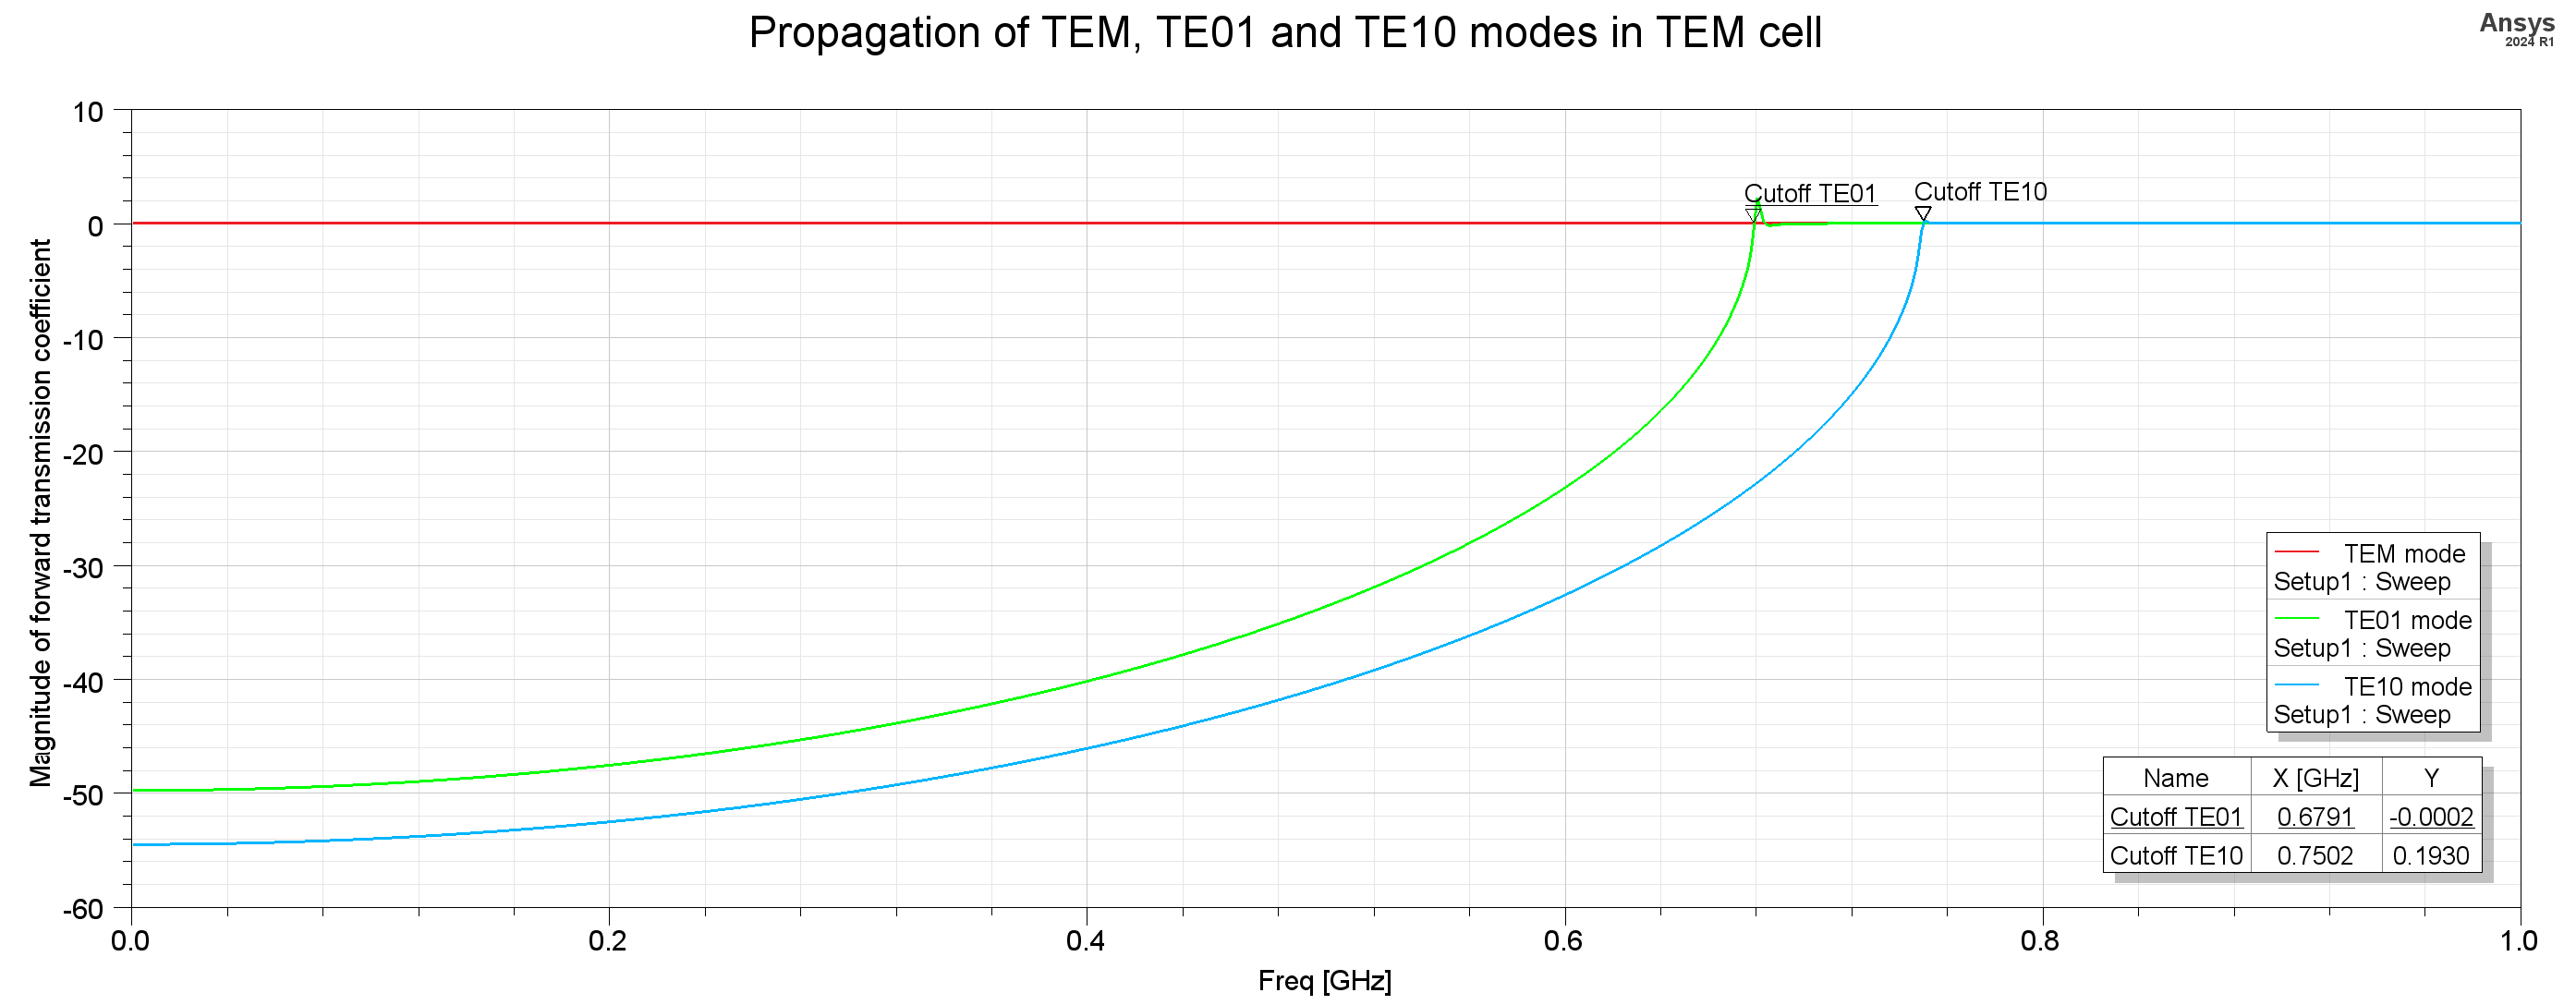
\includegraphics[width=1\linewidth]{Documentation//content//10_theory//img/te01_te10_tem_propagation.png}
    \caption{Propagation of TEM, TE\textsubscript{01} and TE\textsubscript{10} modes in TEM cell}
    \label{fig:te01_te10_tem_propagation}
\end{figure}




The TEM cell does not only support TEM modes, above their cut-off frequency TE and TM modes begin to propagate. Because the TEM cell is a high-Q cavity, those cut-off frequencies are sharply defined frequencies. Due to imperfections, change in materials or finite conductivity of the conducting plates, wave propagating in the TEM mode may excite higher order TE and TM modes, too \cite{10791592}. A change in material, for example, demands the electric and magnetic field to have a component in the direction of propagation at the discontinuity. A paper by Wilson and Ma present analytical approximations to determine these frequencies \cite{Wilson_Ma_1986}.  There is a long list for the several first few corner frequencies of the first modes. Additionally, a paper by Koch, Groh and Garbe determines the resonance frequencies of the first TE modes analytically \cite{10791592}. The TEM mode is necessarily excited by the geometry of the TEM cell, hence this mode is called essential. The higher order TE and TM modes, which are only excited due to non-uniformity of the TEM cell, are called non-essential modes \cite{990711}.


The first modes propagating after the TEM mode is the TE\textsubscript{10} and TE\textsubscript{01} modes. Their transversal electric fields are depicted in \autoref{fig:transversal_e_fields_tem_cell}. 

\begin{figure}[h]
    \centering
    \begin{subfigure}[b]{0.3\linewidth}
        \centering
        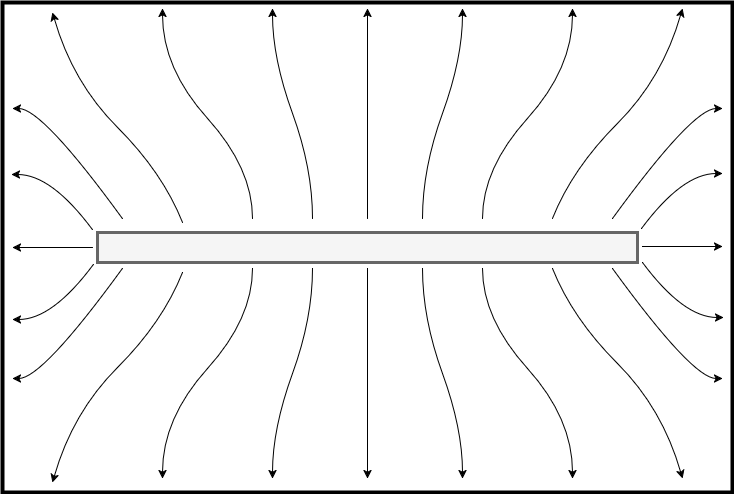
\includegraphics[width=\linewidth]{Documentation/content/10_theory/img/tem_cell_mode.png}
        \caption{TEM Mode}
        \label{fig:tem_mode}
    \end{subfigure}
    \begin{subfigure}[b]{0.3\linewidth}
        \centering
        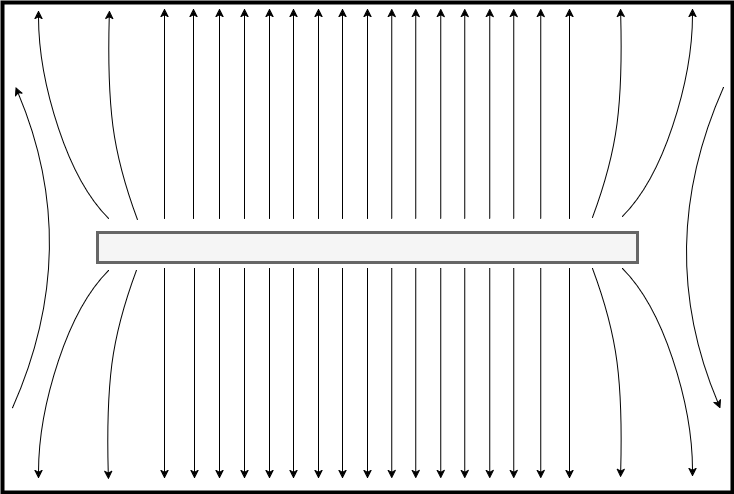
\includegraphics[width=\linewidth]{Documentation/content/10_theory/img/te01_mode.png}
        \caption{TE\textsubscript{01}}
        \label{fig:te01_mode}
    \end{subfigure}
    \begin{subfigure}[b]{0.3\linewidth}
        \centering
        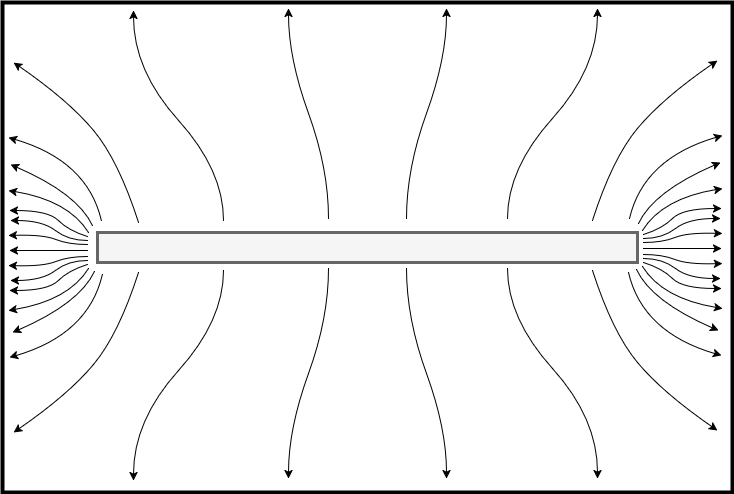
\includegraphics[width=\linewidth]{Documentation/content/10_theory/img/te10_mode.png}
        \caption{TE\textsubscript{10}}
        \label{fig:te10_mode}
    \end{subfigure}
    \caption{Transversal electric fields in cross section of TEM cell}
    \label{fig:transversal_e_fields_tem_cell}
\end{figure}
\todo{Vector directions are wrong in the pictures}




\subsection{Electrically Small Radiating Sources in TEM Cells}

% What is this subsection for? Maybe it should be combined with the TEM cell section. In there, the calculations with Green's theorem and Lorentz Reciprocity Theorem could be put. Then, the calculations from the paper of Sreenivasia could follow. It shows how to find the equivalent Dipole moments. It is important to know which modes are propagating. A Electric dipole, which points in direction of wave propagation, should not influence the result. However, it could create TM modes, which would transfer power to the ports. -> Investigate modes.

An electrically small radiating source may be represented by six dipoles. This number includes three magnetic dipoles pointing in every direction of the Cartesian coordinate system (x, y, and z-direction), and three electric dipoles in the same orientation. Consequently, an equipment under test (EUT) could be modeled with these dipoles, leading to much less computational effort in simulation. The excited EM waves by point sources is discussed in \cite{Collin_2015} and in \autoref{sec:modes_tem_cell}. An analytical procedure to determine these dipole moments is presented by Sreenivasiah \cite{Sreenivasiah_Chang_Ma_1981}, and some experimental results based on it can be found in the research of Kreindl, where bond wires were modeled with magnetic dipoles\cite{Kreindl_Bauernfeind_Weiss_Stockreiter_Kaltenbacher_2024}, and, again, Sreenivasiah \cite{Sreenivasiah_Chang_Ma_1981}.

% Citing: "If the waveguide walls are perfectly conducting, the coefficients of such an expansion may be obtained in a straightforward manner, by an application of Lorentz's reciprocity principle." - This should be treated in the section about TEM cells. A reference to the Lorentz Reciprocity Theorem shall be made, and how it is used to determine the coefficients of the orthonormal modes.

The idea is to place the EUT in the TEM cell and measure the power of both output ports. The amplitudes of the TEM fields are expressed by \autoref{eqn:a_b_moments} \cite{Sreenivasiah_Chang_Ma_1981}. % maybe cut out this equation.

\begin{equation}
    \begin{pmatrix}a \\b\end{pmatrix} = \frac{1}{2}(-\mathbf{m_e}\cdot \mathbf{E_0}^\pm+\mathrm{i}\omega\mu_0\mathbf{m_m}\cdot\mathbf{H_0}^\pm)
    \label{eqn:a_b_moments}
\end{equation}

The magnetic field $\mathbf{H_0}$ and electric field $\mathbf{E_0}$ are both normalized to $1\,\sqrt{\mathrm{Hz}}$ \cite{Kreindl_Bauernfeind_Weiss_Stockreiter_Kaltenbacher_2024} and correspond to the TEM mode in free space \cite{Sreenivasiah_Chang_Ma_1981}. The electric dipole moment $\mathbf{m_e}$ and the magnetic dipole moment $\mathbf{m_m}$ are complex vectors, containing an amplitude and phase for every one of the three directions in the coordinate system (x, y, z), and have the units $\mathrm{A\cdot m}$ and $\mathrm{V\cdot m}$. The variables $a$ and $b$ correspond to the amplitudes of the waves in both possible directions in the TEM cell with the unit $\sqrt{\mathrm{W}}$.
This leads to the final form in \autoref{eqn:a_b_moments_simp} \cite{Sreenivasiah_Chang_Ma_1981}.

\begin{equation}
    \begin{pmatrix}a \\b\end{pmatrix} =-\frac{1}{2}(\mathbf{m_e\pm \mathrm{i}k\mathbf{m_m}\times \mathbf{z})\cdot \mathbf{e_0}}
    \label{eqn:a_b_moments_simp}
\end{equation}

The unity vector $\mathbf{z}$ points in direction of propagation. The function vector $\mathbf{e_0}$ describes the normalized electric field amplitude in traverse direction, i.e. x and y-directions, of the excited fundamental mode. Due to the normalization of the electric and magnetic fields to $1\,\sqrt{\mathrm{W}}$, the total power at one port is 1\,W. This defines $\mathbf{e_0}$ as the electric field when the TEM cell is excited with a peak unit power, since the amplitude of the electric field is considered, not the RMS value.
\todo{peak power, not average. Explain better.}

Note, that an electric dipole in the TEM cell leads to a increase in power with the same phase in both ports, and a magnetic dipole leads to the same increase, but with a phase shift of 180°. This also explains why the EUT shall be place halfway on the septum in x-direction. Any shift from this position changes this phase shift from 180°. It is therefore required to measure the power of the ports with phase information, like using a complex Poynting vector, which is easy to implement in a simulation software. When measuring a device with a real TEM cell, the phase information may be found by summing and subtracting the output powers of the ports, as is shown in \cite{Sreenivasiah_Chang_Ma_1981}.

Additionally, only the electric or magnetic dipole moment, that is aligned with the electric or magnetic field in the TEM cell, influences the output power, ideally. 
% In reality, at frequencies over cut-off frequencies of TE and TM modes, the dipoles not aligned with the TEM mode will generate some TE/TM modes, which enable them to transmit power and disturb the results, as in \cite{Kreindl_Bauernfeind_Weiss_Stockreiter_Yenumula_Narayanan_Kaltenbacher_2022}. 
Furthermore, in the optimal case, the EUT is placed in the dead center of the TEM cell, where the x- and z-component of $\mathbf{e_0}$ in the y=0 plane becomes zero due to symmetry \cite{Sreenivasiah_Chang_Ma_1981}. If this is not the case, the measurements may vary significantly \cite{Kreindl_Bauernfeind_Weiss_Stockreiter_Yenumula_Narayanan_Kaltenbacher_2022}.

The formula has originally been derived for cylindrical waveguides \cite{Collin_2015}. There, the position of the electric and magnetic dipole moments do not matter, as long as the matching electric and magnetic fields at the surfaces are chosen. This is because the field components do not change direction when propagating from the dipoles to the surfaces, due to the symmetrical property of the cylindrical waveguide. This is not the case for a TEM cell. There, an offset into the x- and y-direction from the center leads to field components, which change direction while traveling to the surfaces. Then, the vector product used in the derivation by Lorentz Reciprocity theorem is not valid anymore. Instead, the fields at the test points have to be considered, and because they don't have a singular x,y or z-component anymore, several more dipole moments become relevant.

However, in a TEM cell, the normalized electric field strength is not necessarily symmetrical. Therefore, it must be found out, depending on the position of the dipole moment. In dead center, the normalized electric field only has a z-component. However, with an offset towards z- or y-direction, it will have a y-component, too. Then, the normalized electric field $\mathbf{e_0}$ can be found with through \autoref{eqn:e0x_mse} for  and \autoref{eqn:e0z_mse}. For these equations, a known electric dipole moment $m_{\mathrm{se}}$ is used for both the x- and z-direction. $P_\mathrm{x}$ and $P_\mathrm{z}$ describe the output powers at one port, depending on the electric dipole's orientation \cite{Sreenivasiah_Chang_Ma_1981}. When knowing the normalized electric field $\mathbf{e_0}$ at this point, any magnitude of electric dipole moments may be derived by scaling the coefficients $a$ and $b$. When only considering dipole moments in z-direction, then only \autoref{eqn:e0z_mse} is needed.

\begin{subequations}
\begin{equation}
    e_{\mathrm{0x}} = \frac{2 \sqrt{P_\mathrm{x}}}{m_{\mathrm{se}}}
    \label{eqn:e0x_mse}
\end{equation}
\begin{equation}
    e_{\mathrm{0z}} = \frac{2 \sqrt{P_\mathrm{z}}}{m_{\mathrm{\mathrm{se}}}}
    \label{eqn:e0z_mse}
\end{equation}
\end{subequations}

The normalized electric field of the TEM mode is then given by \autoref{eqn:eox_normalized} in x-direction and by \autoref{eqn:eoz_normalized} in z-direction \cite{Wilson_Ma_1986}. The equations follow from the singular integral-equation approach in \cite{Wilson_1981}. The formula is not valid for the gap regions. However, since there isn't any dipole moment to expected there, it should still suffice. 

\begin{subequations}

\begin{equation}
    e_{ox} = \frac{2}{a} Z_c^{1/2} \sum_{m_0=1}^{\infty} 
    \frac{\sinh M(b - pz)}{\sinh M b} 
    \cdot \sin Mx \sin Ma \; J_0(Mg)
    \label{eqn:eox_normalized}
\end{equation}


\begin{equation}
    e_{oz} = p\,\frac{2}{a}\, Z_c^{1/2} \sum_{m_0=1}^{\infty}
    \frac{\cosh M(b - pz)}{\sinh M b}
    \cdot \cos Mx\, \sin Ma\, J_0(Mg)
    \label{eqn:eoz_normalized}
\end{equation}
    
\end{subequations}

$Z_\mathrm{c}$ is the characteristic wave impedance, $a$ is half the width of the TEM cell, $b$ is half its height. The sign-function $p=1$ above the septum, and $p=-1$ below it. $M=m\pi / 2a$ and $g$ is the length of the gap between the septum and the conducting wall. The index $m=1,3,5, ...$ is iterated over odd integers. 

\begin{figure}[h]
    \centering
    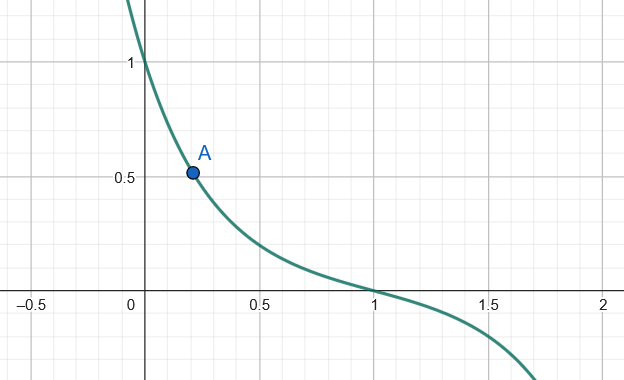
\includegraphics[width=0.5\linewidth]{DELETE2.png}
    \caption{Normalized e-field distribution along z-axis at center of septum}
    \label{fig:placeholder}
\end{figure}

\todo{The electric field / magnetic field distribution of the TEM mode must be known ($e_0$). Other mode distributions are neither available, nor necessary. Calculations to find these field distributions can be found in \cite{4091811}. This would also solve the problem with not being able to shift the location of the electric dipole moment. In \cite{Sreenivasiah_Chang_Ma_1981}, the normalized electric field was also determined analytically, just with output power. IMPORTANT!!! Additionally, the electric field at the output port and the dipole location must be equal (in tem mode) for the formula to work. If they are not, then the formulas derived in \cite{4091811} must be used. That's why the formula does not work for offset shift of the dipole moment anymore. The electric field at the incident port must then be found out. How to use this in case of a shielding material? Not valid for only ez dipole}

% The paper goes on to talk about the total power radiated by the EUT in free space. I don't think I need that, but this comment is here as a reminder that it exists.


\subsection{Shielding}

Effective shielding is of great interest to reduce EMI of electronic systems. A figure of merit for shielding capabilities of a material is the electromagnetic shielding effectiveness (SE), given in \autoref{eqn:se_elec_fields} \cite{10518640}. $E_\mathrm{i}$ is the incident electric field, while $E_\mathrm{t}$ is the transmitted electric field, also depicted in \autoref{fig:shielding_material_diagram}. It depends on the thickness and shape of the material, and its electric and magnetic properties. Additionally, the TEM cell contributes to the SE values.

% Should I add wave reflections formula?

\begin{equation}
    SE_{\mathrm{dB}}=20\log{(\frac{E_\mathrm{i}}{E_\mathrm{t}})}
    \label{eqn:se_elec_fields}
\end{equation}

\begin{figure}[h]
    \centering
    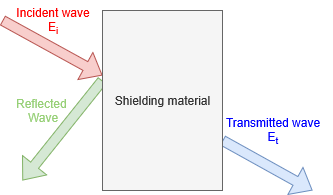
\includegraphics[width=0.35\linewidth]{Documentation//images/shielding_material_diagram.png}
    \caption{Incident, reflected and transmitted electric fields due to interaction with shielding material}
    \label{fig:shielding_material_diagram}
\end{figure}

% (Note: Higher order modes may be able to propagate in the TEM cell, as the refraction of the shielding material follows to excitation of these modes.)

An electromagnetic wave may undergo several reflections inside the shielding material, with each reflection adding up to the total reflected, absorbed and transmitted waves. The total shielding effectiveness is therefore determined by \autoref{eqn:se_rereflections}, according to Schelkunoff. $A_{\mathrm{dB}}$ represents the absorption losses traveling through the shield, $R_{\mathrm{dB}}$ the reflection losses, and $B_{\mathrm{dB}}$ is the correction factor for the multiple reflections inside the shield \cite{10518640}.

\begin{equation}
    SE_{\mathrm{dB}}=R_{\mathrm{dB}}+A_{\mathrm{dB}}+B_{\mathrm{dB}}
    \label{eqn:se_rereflections}
\end{equation}

Calculate with S-params $S_{11}$ and $S_{21}$: A, R and T.  

This approach to shielding with internal re-reflections in the shielding material was derived by Schelkunoff. 
\url{https://www.ieee.li/pdf/viewgraphs/fundamentals_electromagnetic_shield.pdf}

The reflections occur due to the change in wave impedance. They are described through a reflection coefficient $R$. Additionally, it is common to normalize the wave impedance $Z$ to the free-space wave impedance $Z_0$. At the interface from free-space to a shielding material, this leads to \autoref{eqn:reflection_coefficient_plane_dielectric} \cite{Collin_2015}. 

\begin{equation}
    R=\frac{Z-1}{Z+1}
    \label{eqn:reflection_coefficient_plane_dielectric}
\end{equation}

\begin{equation}
    Z=\frac{1}{Z_0}\sqrt{\frac{\mathrm{i}\omega\mu}{\sigma+\mathrm{i}\omega\epsilon}}
    \label{eqn:rel_wave_imp}
\end{equation}

The reflection coefficient can be converted into dB, leading to $R_\mathrm{dB}$. Any additional reflection happen due to re-reflections inside the shielding material, described by $B_\mathrm{dB}$. The rest of the energy must either be absorbed, described by $A_\mathrm{dB}$ or transmitted, shown by $T_\mathrm{dB}$. 

\todo{p. 309 Classical Electrodynamics (John David Jackson) describe shielding material by dipole moments}

The wave number $k$ in lossy media is described in a real an imaginary parts as in \autoref{eqn:wave_number}. The imaginary part $\alpha$ is the attenuation or absorption coefficient. It describes the reduction of the intensity of the wave, which occurs with $\mathrm{e}^{-\alpha x}$, where x is the coordinate direction of propagation. The real part $\beta=\frac{2\pi}{\lambda}$ is the phase constant \cite{Jackson}.

\todo{Formula $\alpha$? Needed?}

\begin{equation}
    k = \beta + \mathrm{i}\frac{\alpha}{2}
    \label{eqn:wave_number}
\end{equation}
\begin{equation}
    \mathbf{E} = \mathbf{e}\cdot \mathrm{e}^{\mathrm{i}kx}
\end{equation}

\todo{S-parameters should enable derivation of $\alpha$. Due to normal incident wave of TEM, no angle needed to consider.}

% Quick mathematical formulation of how to calculate reflected waves?

\todo{Basics: Balanis 2012 page 68?}

When the molecules in a material are exposed to electric fields, they will polarize, described by their permittivity $\epsilon$. When exposed to a magnetic field, the spinning of their electrons in the atoms align with the magnetic field, described by the permeability $\mu$ of the material. When the fields alternate over time, the molecules will always move and align according to them. This is essentially a movement of charges, and therefore described by a conductivity $\sigma$. The energy lost in this process is dissipated as heat \cite{Balanis_2012}.

The electric field will push charges in polarizable molecules apart. This separation of charges may be described as a electric dipole, depending on the separation distance and the charge. Under alternating electric fields, the moving of charges will contribute to $\sigma$. This phenomenon is called dielectric hysteresis. \autoref{eqn:loss_tangent_permittivity} quantifies it by a loss tangent $\tan\delta_e$ \cite{Balanis_2012}. There, $\sigma_s$ is the static conductivity, meaning the conductivity of the material for static fields. The complex part of the permittivity $\epsilon''$ describes the lossy part of the dielectric material, specifically relevant for the alternating fields case. The real part of the permittivity is lossless and is noted by $\epsilon'$. The overall complex permittivity is therefore $\epsilon=\epsilon'+\mathrm{i}\epsilon''$.
\todo{Some way to describe coupling of shielding material to TEM cell?}

\begin{equation}
    \tan\delta_e = \frac{\sigma_s}{\omega\epsilon'}+\frac{\epsilon''}{\epsilon'}
    \label{eqn:loss_tangent_permittivity}
\end{equation}

The loss tangent therefore $\tan\delta_e$ relates the conductivity of a material to the real permittivity. A dielectric with low losses has a much larger displacement current than conduction current density ($\tan\delta_e \ll 1$). The opposite is true for a good conductor ($\tan\delta_e \gg 1$) \cite{Balanis_2012}.

The loss tangent $\tan\delta_e$ is a function of frequency, however, it is often not stated as such. Therefore, the loss tangent of FR4, for example, is given as $\tan\delta_e=0.02$ for frequencies up to 1\,GHz. For higher frequencies, the molecules may have resonance frequencies, where they influence more strongly the overall conductance and consequently increase the imaginary part of the permittivity $\epsilon''$.

There are also magnetically lossy materials, which is introduced by a complex permeability $\mu=\mu'+\mathrm{i}\mu''$. Analog to the dielectric case, the permeability can also be described by a loss tangent $\tan{\delta_m}$ as shown in \autoref{eqn:magnetic_loss_tangent}. However, the loss tangent is very low for the majority of materials and will be neglected. Ferrites are an exception, which are commonly used to dampen high frequency signals \cite{Balanis_2012}.

\begin{equation}
    \tan{\delta_m}=\frac{\mu''}{\mu'}
    \label{eqn:magnetic_loss_tangent}
\end{equation}


\todo{describe $\alpha$ and $\delta$ for absorption. Then reflections with $\epsilon$ and $\mu$}

\subsubsection{ASTM ES7-83 Method}

The ASTM ES7-83 method is used to determine the shielding effectiveness of shielding materials. The shielding material is inserted into a coaxial TEM cell around the septum. Ideally, they form a continuous connection \cite{MORARI_BĂLAN_2015}. 

In this method, two measurements are performed with an oscilloscope attached to the output of the TEM cell. In the first, an empty TEM cell is excited and a reference output voltage $U_\mathrm{ref}$ is measured. In the second, the TEM cell is loaded with the shielding material, and the output voltage $U_\mathrm{load}$ is again noted. The measurement values are then used in \autoref{eqn:SE_voltages} to derive the shielding effectiveness $SE_\mathrm{dB}$ \cite{MORARI_BĂLAN_2015}.

\begin{equation}
    SE_\mathrm{dB}=20\cdot\log{\left(\frac{U_\mathrm{ref}}{U_\mathrm{load}}\right)}
    \label{eqn:SE_voltages}
\end{equation}

In the case of simulating the problem, such a procedure may be used, too. It is more convenient, then, to defined a reference output power $P_\mathrm{ref}$ for an unloaded TEM cell, and a output power for the loaded case $P_\mathrm{load}$. This leads to the similar \autoref{eqn:SE_power}.

\begin{equation}
    SE_\mathrm{dB}=10\cdot\log{\left( \frac{P_\mathrm{ref}}{P_\mathrm{load}} \right)}
    \label{eqn:SE_power}
\end{equation}

Additionally, a rectangular TEM cell is used for this method, instead of the commonly used cylindrical version. \autoref{fig:form_of_shielding_material} shows the cross section of this shielding material, which is inserted into the TEM cell. In \autoref{fig:ASTM ES7-83} the shielding material can be seen wrapped around the septum. 

\begin{figure}[h]
    \centering
    \begin{subfigure}[h]{0.49\textwidth}
        \centering
        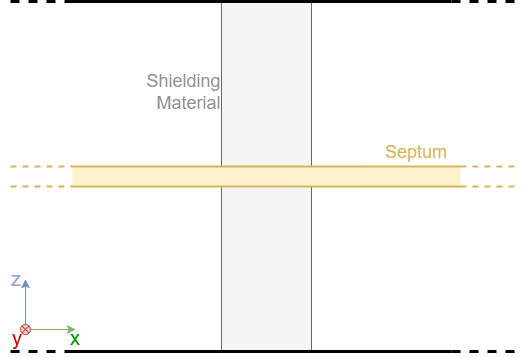
\includegraphics[width=\textwidth]{Documentation//content//10_theory//img/ASTM ES7-83.png}
        \caption{Shielding material in TEM cell}
        \label{fig:ASTM ES7-83}
    \end{subfigure}%
    \hfill
    \begin{subfigure}[h]{0.49\textwidth}
        \centering
        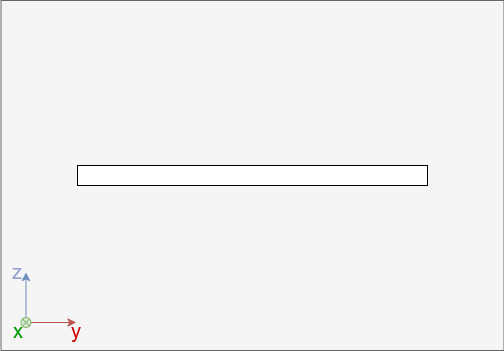
\includegraphics[width=\textwidth]{Documentation//content//10_theory/img/form_of_shielding_material.png}
        \caption{Shape of the shielding material}
        \label{fig:form_of_shielding_material}
    \end{subfigure}
    \label{fig:subfigures}
\end{figure}

Then, the S-parameters derived in the simulations are used to get to the output powers $P_\mathrm{ref}$ and $P_\mathrm{load}$. By exciting the TEM cell with a power of 1\,W, the reference power $P_\mathrm{ref}=1\,\mathrm{W}$. The measured power is then derived through \autoref{eqn:load_power}.

\begin{equation}
    P_\mathrm{load}=P_\mathrm{ref}\cdot10^{|S_\mathrm{12}|/10}
    \label{eqn:load_power}
\end{equation}


\todo{Describe Method. Then follows dual TEM cells}


\section{Antennas}
\subsection{Antennas to Investigate}

% List possible electrically short antennas to investigate with dipole moments here. Describe, why they are interesting.
% See: Crossed Dipole Antennas document by Bauernfeind

\subsubsection{IFA}
\subsubsection{Center fed monopole antenna
\subsection{Crossed dipole antenna}
\begin{figure}[h]
    \centering
    \includegraphics[width=0.5\linewidth]{crossed_dipole_antenna.png}
    \caption{A crossed dipole antenna \cite{7293591}}
    \label{fig:placeholder}
\end{figure}

A crossed dipole antenna radiates very evenly into every direction. This could be interesting to use, in order to excite several modes, especially in the presence of shielding materials.

When this antenna is near a perfect electric conductor (PEC), the gain becomes dependent on the distance to it. At a distance of $H=0.25\lambda$, the gain reaches a maximum due to constructive interference in normal direction to the PEC surface. When the distance is small, the image currents may cancel and the gain decreases. Therefore, the output power on the TEM cells depends on the distance, and implicitly on the frequency. This means that the frequency behavior of the representing dipoles may vary from a standard dipole.

Additionally, when a shielding material is present, different modes may be excited, which also influence the behavior. Those different modes depend on all 6 dipole moments, with which the antenna shall be modeled. 


\section{Simulations}\label{sec:simulations}



\subsection{Inverted F-antenna}\label{sec:ifa_sim}




The inverted F-antenna (IFA) is modeled in Ansys HFSS as shown in \autoref{fig:ifa}. Its material is copper. It is positioned at the center of the TEM cell, mounted at the top surface. The 5\,mm long wire points towards waveport 2. The excitation is a modal wave port. With a maximum dimension of 5\,mm, the antenna is electrically small for a frequency of up to 6\,GHz, at which it will be a tenth of the wavelength. In this simulation, the antenna is investigated for the frequency of 100\,MHz to 1\,GHz. The TEM cell has a width of 40\,mm and a height of 24\,mm. The goal is to find equivalent dipole moments. 


\begin{figure}[h]
    \centering
    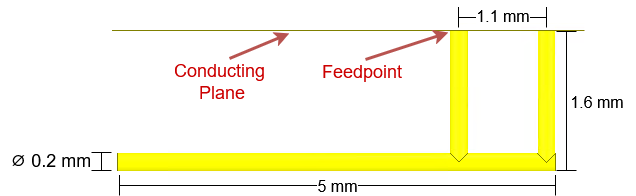
\includegraphics[width=0.75\linewidth]{Documentation//content//30_simulations//img/inverted_f_antenna.png}
    \caption{Inverted F-antenna used in the simulation}
    \label{fig:ifa}
\end{figure}

The coupling between the antenna and the two ports of the TEM cell are described by S-parameters, specifically the forward transmission coefficients $S_{\mathrm{A1}}$ and $S_{\mathrm{A2}}$. \autoref{fig:antenna_waveport1_sparams} shows the magnitude of this coefficient, which is the same for the antenna to both ports. The phase shifts of $S_{\mathrm{A1}}$ and $S_{\mathrm{A2}}$ differ, which is shown in \autoref{fig:phase_shift_waveports_ifa}. This phase shift delivers important information about the equivalent dipole moments.
 

\begin{figure}[h]
    \centering
    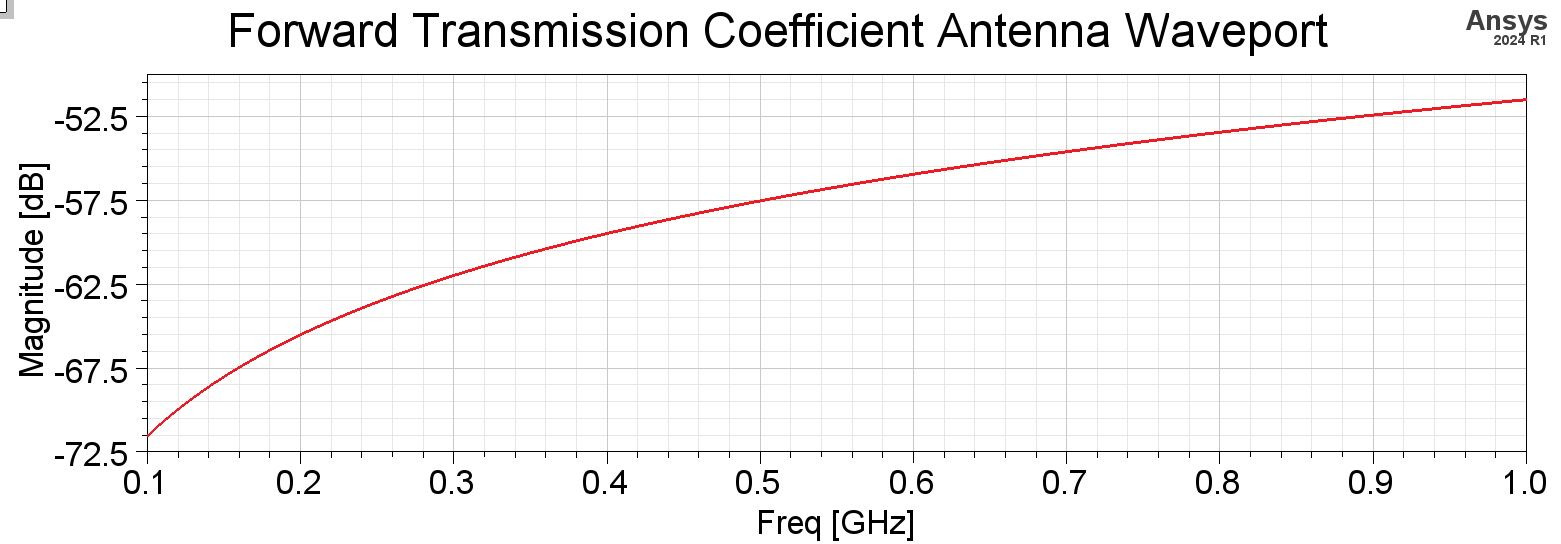
\includegraphics[width=1\linewidth]{Documentation//content//30_simulations//img/antenna_waveport1_sparams.png}
    \caption{S-Parameter describing coupling of antenna to waveport 1}
    \label{fig:antenna_waveport1_sparams}
\end{figure}

\begin{figure}[h]
    \centering
    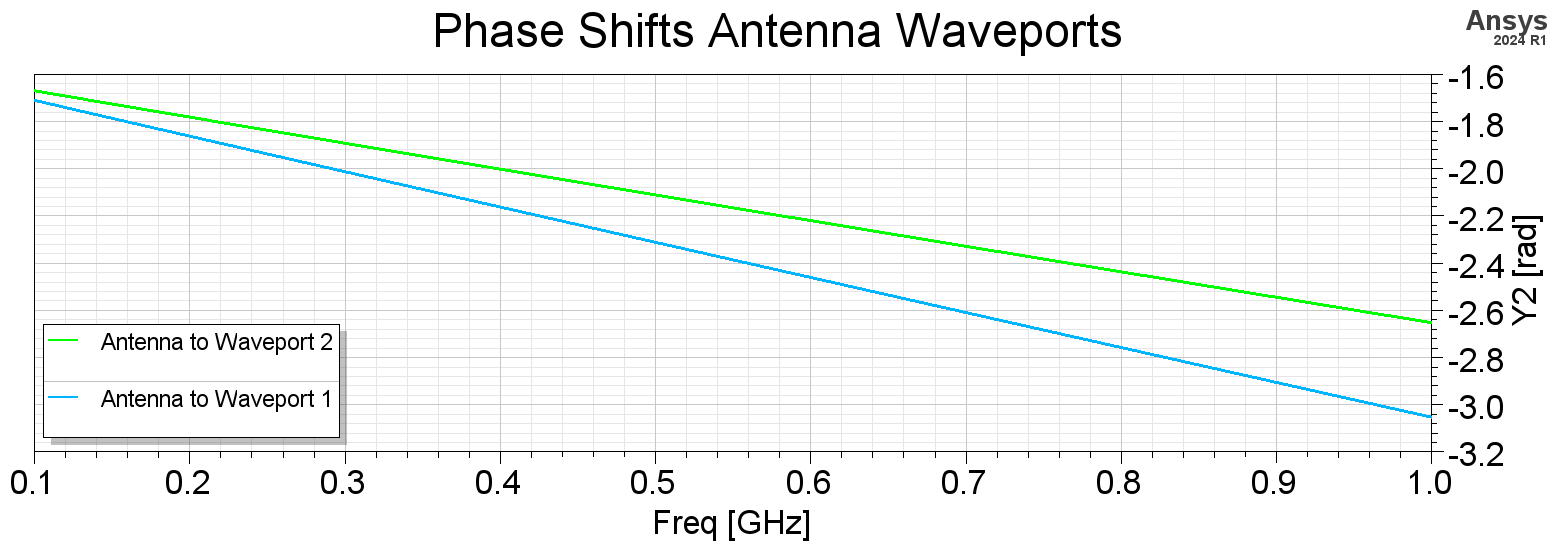
\includegraphics[width=1\linewidth]{Documentation//content//30_simulations//img/Phase Shift Waveports.png}
    \caption{Phase of S-parameters from antenna to waveport 1 and 2}
    \label{fig:phase_shift_waveports_ifa}
\end{figure}


\begin{equation}
    P_{\mathrm{Antenna}}=\frac{P_{\mathrm{Out1}}}{10^{|S_{\mathrm{A1}}|/10}}=\frac{P_{\mathrm{Out2}}}{10^{|S_{\mathrm{A2}}|/10}}
    \label{eqn:power_antenna}
\end{equation}


\autoref{eqn:power_antenna} describes the relation between the input power at the antenna and the measured output power of the TEM cell. It is defined by the magnitude of the forward transmission coefficients.

\begin{equation}
    \iint_A \mathbf{e_0} \times \mathbf{h_0} \cdot\mathrm{d}\mathbf{A} = 1
    \label{eqn:normalization of fields}
\end{equation}

\autoref{eqn:normalization of fields} shows that the electric field $\mathbf{e_0}$ and magnetic field $\mathbf{h_0}$ are normalized to $1\,\sqrt{\mathrm{W}}$. The surface area $A$, over which the fields are integrated, is that of the output ports of the TEM cell. The field can be linearly scaled by the coefficients $a$ and $b$, which has been described in \autoref{eqn:modal_superposition1} and \autoref{eqn:modal_superposition2}. Only one pair of such coefficients is needed, since only the TEM mode is considered. The coefficients $a$ and $b$ have the unit $\sqrt{\mathrm{W}}$. The fields $\mathbf{e_0}$ and $\mathbf{h_0}$ are not known over the whole area. However, the electric field $\mathbf{e_0}$ has only to be known at one specific point in order to determine the equivalent dipole moments, as will be shown here.

\begin{subequations}
\begin{equation}
    P_{\mathrm{out1}}=\iint_A \langle \mathbf{S} \rangle \cdot \mathrm{d}\mathbf{A}= \iint_A \frac{1}{2} \, \Re \{ \left(a\cdot \mathbf{e_0}\right) \times \left(a\cdot \mathbf{h_0}^*\right) \}\cdot \mathrm{d}\mathbf{A} = \frac{|a|^2}{2}
    \label{eqn:power_of_poynting1}
\end{equation}
\begin{equation}
    P_{\mathrm{out2}}=\iint_A \langle \mathbf{S} \rangle \cdot \mathrm{d}\mathbf{A}= \iint_A \frac{1}{2} \, \Re \{ \left(b\cdot \mathbf{e_0}\right) \times \left(b\cdot \mathbf{h_0}\right)^* \}\cdot \mathrm{d}\mathbf{A} = \frac{|b|^2}{2}
    \label{eqn:power_of_poynting2}
\end{equation}
\end{subequations}
\todo{linear relation Power to b, a}

The output power of each port is then derived through \autoref{eqn:power_of_poynting1} and \autoref{eqn:power_of_poynting2}. So if $a=b=1$, then the electric field $\mathbf{e_0}$ may be measured, when the output power at one port is $\frac{1}{2}\,\mathrm{W}$. Because it is assumed that the TEM cell contains only waves in the TEM mode, the normalization of the electric and magnetic fields can be used to simplify the calculations.

\begin{equation}
    \mathbf{e_0}\times\mathbf{h_0}=\Re\{\mathbf{e_0}\times\mathbf{h_0}^*\} \quad\text{for TEM mode}
    \label{eqn:equivalent_tem}
\end{equation}

\todo{Problem with large TEM cell: Formula does not work for large frequencies. The field distributes around the port. Describe this. Error grows with frequency}

By using \autoref{eqn:mag_dipole_moment_tem} and \autoref{eqn:dipole_tem_waves}, the equivalent dipole moments are derived. Because of Lorentz reciprocity theorem, only fields aligned with the dipole moments get to the output ports. Since only the TEM mode propagates, only the electric dipole moment in z-direction and the magnetic dipole moment in y-direction influence the fields. If higher order modes can propagate, the other dipole moments become relevant, too.
\todo{Einheitliches Koordinatensystem definieren}



\begin{equation}
    m_{\mathrm{e}}=\frac{a+b}{e_{0,z}}
    \label{eqn:ifa_me}
\end{equation}

\begin{equation}
    m_{\mathrm{m}}=\mathrm{i}\frac{a-b}{k_0  e_{0,z}}
    \label{eqn:ifa_mm}
\end{equation}

By adding or subtracting the coefficients $a$ and $b$, the dipole moments are expressed into the handy \autoref{eqn:ifa_me} and \autoref{eqn:ifa_mm}. There, $k_0=\frac{2\pi}{\lambda}$ is the free space wave number and $e_{0,z}$ is the normed electric field in z-direction at middle height between septum and the upper wall of the TEM cell. However, the exact height of the measurement point is not important, as the electric field is uniformly distributed. Additionally, the x- and y-components of the electric field $\mathbf{e_{0}}$ are defined to be zero, which leads to these equations. The dipole moments $m_{\mathrm{e}}$ and $m_{\mathrm{m}}$ are defined to be in the center of the TEM cell, at middle height. If they are shifted in any direction, their approximation would not hold true anymore.

\begin{figure}[h]
    \centering
    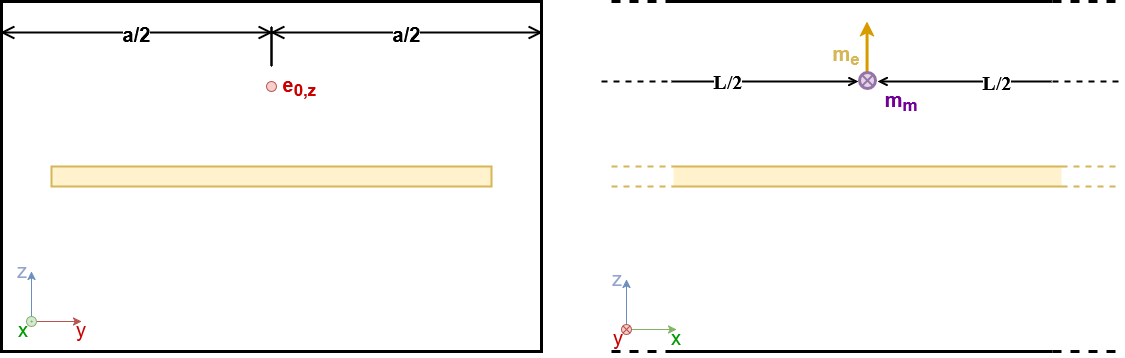
\includegraphics[width=1\linewidth]{Documentation//content//30_simulations//img/sketch_dipoles_tem_cell.png}
    \caption{Dipole moments and measurement point of $e_{0,z}$ in TEM cell}
    \label{fig:sketch_dipoles_tem_cell}
\end{figure}

Using \autoref{eqn:magn_current_curr_loop} the magnetic dipole moment can be expressed as a magnetic current. The resulting $m_{m,mag}$ is shown in \autoref{eqn:m_mymag_ifa}. The phase shift between the magnetic and electric dipole moments $m_{\mathrm{ez}}$ and $m_{\mathrm{my,mag}}$ is always $\frac{\pi}{2}$, which generates the desired TEM wave pattern.

\begin{equation}
    m_{\mathrm{m,mag}}=\mathrm{i}m_{\mathrm{m}}\omega\mu_0
    \label{eqn:m_mymag_ifa}
\end{equation}

The antenna may then be replaced with those two dipole excitations in the center of the upper half of the TEM cell. The magnitude and phase of the fields, as well as the output powers, should remain the same as in the case with the antenna. 

\begin{figure}[h]
    \centering
    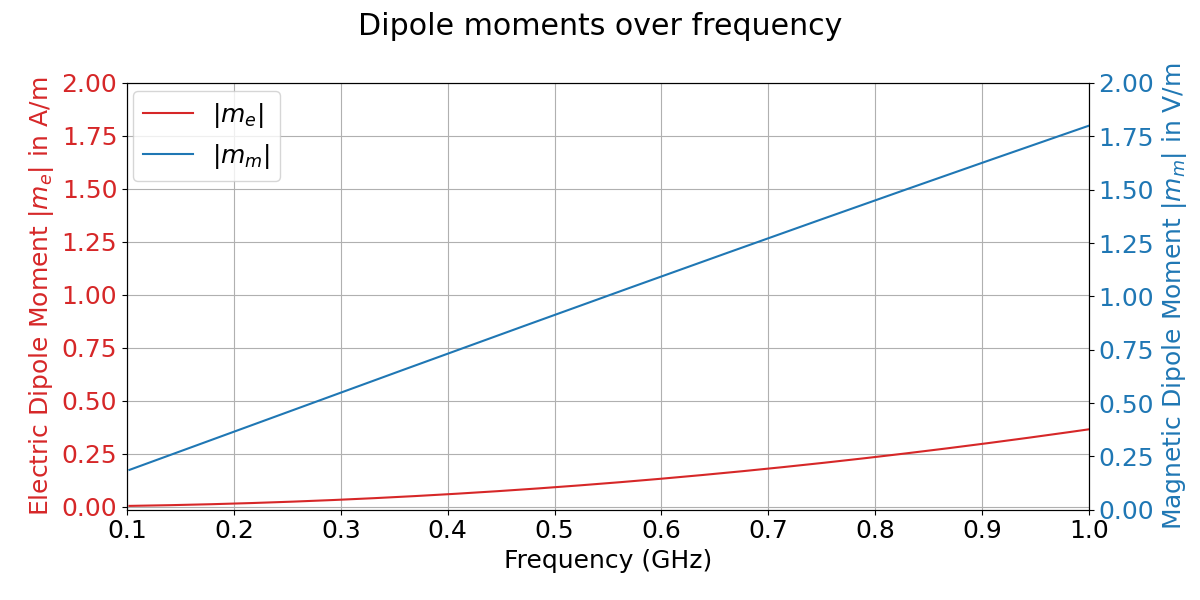
\includegraphics[width=1\linewidth]{Documentation/content/30_simulations/img/dipole_moments_over_freq_ifa.png}
    \caption{Dipole moments over frequency}
    \label{fig:dipole_moments_over_freq_ifa}
\end{figure}

\autoref{fig:dipole_moments_over_freq_ifa} shows the dipole moments over frequency. The electric dipole moment $m_e$ has been normalized to the free-space wave impedance of $377\,\Omega$ to make the dipole moments comparable. The antenna input power has been set to 142588.47\,W, because this leads to an output power of 1\,W at a frequency of 1\,GHz. The magnetic dipole moment is much larger than the electric dipole moment, because the current loop of the antenna is aligned with the TEM cell's magnetic fields, but the line current is not with the TEM electric fields. The magnetic dipole moments rises linearly with the frequency, which is equal to a quadratic increase of power. Only the TEM modes has been considered in the simulation, as other modes disturb the calculations. 

The electric field $\mathbf{e_0}$ is approximated with \autoref{eqn:ifa_e_field_approx} for the purpose of interpolation over frequencies and analytical analysis. \autoref{fig:output_power_e_fields_over_freq_ifa} shows the resulting plot. If any other output power over frequency curves are desired, the formula may easily be modified by considering the quadratic relationship between the electric field and the output power.

\begin{equation}
    a\cdot\mathbf{e_0}=\frac{\sqrt{P_\mathrm{Out}}}{0.0012194}\,\mathrm{\frac{V}{m\sqrt{W}}}
    \label{eqn:ifa_e_field_approx}
\end{equation}

\begin{figure}[h]
    \centering
    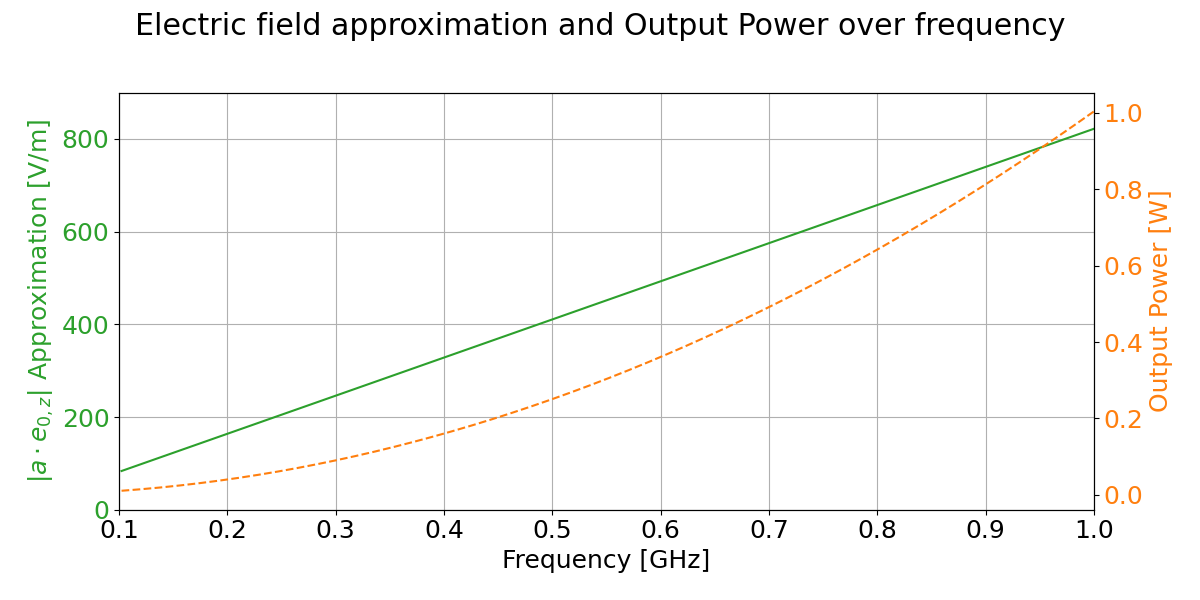
\includegraphics[width=1\linewidth]{Documentation//content//30_simulations//img/output_power_e_fields_over_freq_ifa.png}
    \caption{Output power and electric field over frequency}
    \label{fig:output_power_e_fields_over_freq_ifa}
\end{figure}

\subsection{Center Fed Monopole Antenna}

\begin{figure}[h]
    \centering
    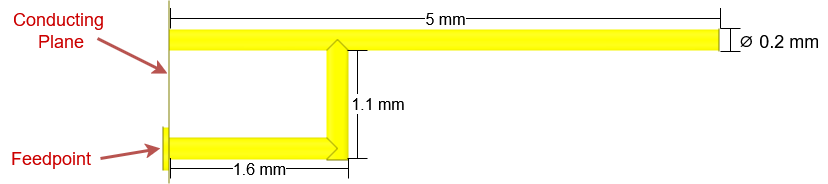
\includegraphics[width=0.75\linewidth]{Documentation//content//30_simulations//img/center_fed_monopole.png}
    \caption{Center fed monopole antenna used in simulation}
    \label{fig:center_fed_monopole}
\end{figure}






\subsection{Offset of source antennas and eddy currents}



\newpage

\iffalse
\subsection{Summary}

\fi
\cleardoublepage
\printbibliography

\end{document}
